\clearpage
\section{Critical algorithms}\label{sec:critical_algorithms}

This section summarizes the status of the critical algorithms that were identified in the Data Reduction Library Specifications document~\cite{DRLS} at PDR. Note that `critical' in this context stands for `needs prototyping', and `non-critical' below does not mean `unimportant', just that there is a reason for not needing a prototype.

\begin{enumerate}
    \item[1.] Persistence correction (\ref{ssec:criticalpersistencecorrection})
    \begin{itemize}
        \item \textit{Reason at PDR}: Persistence is a major issue in modern IR detectors, and the determination of this pattern relies on observations previously done, which might arise from completely other observing runs and are therefore proprietary.
        \item \textit{Status at FDR}: The persistence correction algorithm will be developed by ESO, making the part in the Data Reduction Library non-critical.
        \item \textit{Prototype delivery}: None
    \end{itemize}
    \item[2.] Detector Masks (\ref{ssec:criticaldetetctormasks})
    \begin{itemize}
        \item \textit{Reason at PDR}: Reason unknown.
        \item \textit{Status at FDR}: Standard procedures apply, therefore not critical.
        \item \textit{Prototype delivery}: None.
    \end{itemize}
    \item[3.] Bad pixel determination (\ref{ssec:criticalbadpixeldetermination})
    \begin{itemize}
        \item \textit{Reason at PDR}: Reason unknown.
        \item \textit{Status at FDR}: Standard procedures apply, therefore not critical.
        \item \textit{Prototype delivery}: None.
    \end{itemize}
    \item[4.] Background subtraction (\ref{ssec:criticalbackgroundsubtraction})
    \begin{itemize}
        \item \textit{Reason at PDR}: A proper background correction is essential to ensure accurate photometric and spectroscopic analysis of the observed sources because observations in the mid-infrared are affected by the high sky and telescope background.
        \item \textit{Status at FDR}: Standard subtraction techniques (dithering, chopping and nodding) will be used, which do not require prototyping. More complex algorithms that would have required prototypes, e.g.~involving principal component analysis, have been ruled out since PDR.
        \item \textit{Prototype delivery}: None
    \end{itemize}
    \item[5a.] LSS Wavelength calibration and distortion correction (\ref{ssec:criticalwavelengthanddistortionlss})
    \begin{itemize}
        \item \textit{Reason at PDR}: A new algorithm is necessary for wavelength calibration and distortion correction for LSS.
        \item \textit{Status at FDR}: We will use the algorithms from PyReduce.
        \item \textit{Prototype delivery}: An adaptation of the PyReduce package.
    \end{itemize}
    \item[5b.] \ac{IFU} Wavelength calibration and distortion correction (\ref{ssec:criticalwavelengthanddistortionifu})
    \begin{itemize}
        \item \textit{Reason at PDR}: A new algorithm is necessary for wavelength calibration and distortion correction for IFU.
        \item \textit{Status at FDR}: Use the same algorithms as for LSS (PyReduce), but via their incarnation in the CRIRES pipeline.
        \item \textit{Prototype delivery}: A JuPyter-notebook with instructions to call the CRIRES pipeline and example input/output files.
    \end{itemize}
    \item[6.] Telluric correction (\ref{ssec:criticaltelluriccorrection})
    \begin{itemize}
        \item \textit{Reason at PDR}: Telluric correction, i.e. the removal of absorption features arising in the Earth’s atmosphere, is a critical issue as the imprint of molecular species present in our air may vary on different timescales down to minutes due to changes in their composition and their amount.
        \item \textit{Status at FDR}: We either use molecfit or a telluric standard star. Both ways are well proven, and therefore we will not deliver a prototype.
        \item \textit{Prototype delivery}: None.
    \end{itemize}
    \item[7.] Error propagation (\ref{ssec:criticalerrorpropagation})
    \begin{itemize}
        \item \textit{Reason at PDR}: Error propagation is important.
        \item \textit{Status at FDR}: The \ac{HDRL} provides standardized mechanisms for error propagation; prototyping is therefore not necessary.
        \item \textit{Prototype delivery}: None.
    \end{itemize}
    \item[8.] N-band image restoration (\ref{ssec:criticalnbandimagerestoration})
    \begin{itemize}
        \item \textit{Reason at PDR}: There is no standard algorithm for extended sources.
        \item \textit{Status at FDR}: The science drivers (AGN and circumstellar disks) are compact enough to treat as point-like, using the VISIR algorithm for compact sources. Extended diffuse objects will be observed with large chop-offset for background subtraction and thus no specific algorithm is necessary.
        \item \textit{Prototype delivery}: None.
    \end{itemize}
    \item[9.] IFU image and cube reconstruction (\ref{ssec:criticalifuimageandcubereconstruction})
    \begin{itemize}
        \item \textit{Reason at PDR}: Due to the width of the slices in the LM integral-field spectrograph of $20.7\,\mathrm{mas}$,
            the PSF is undersampled in the across-slice direction, and there is no known cube reconstruction algorithm.
        \item \textit{Status at FDR}: A prototype algorithm is implemented in Python.
        \item \textit{Prototype delivery}: Python package.
    \end{itemize}
    \item[10.] IFU data rate (\ref{ssec:criticalifudatarate})
    \begin{itemize}
        \item \textit{Reason at PDR}: For very bright sources, short exposures result in high data rates which may present a problem for
            the observatory pipeline which has to deal with the data in real time.
        \item \textit{Status at FDR}: The data rate is under control and does not require prototyping.
        \item \textit{Prototype delivery}: None.
    \end{itemize}
\end{enumerate}

The following additional critical algorithms were identified in the period between PDR and FDR:

\begin{enumerate}
    \item[11.] ADI algorithm (\ref{ssec:criticaladialgorithm})
    \begin{itemize}
        \item \textit{Reason at FDR}: Considering many of the science cases for METIS are focusing on direct imaging / high contrast imaging we deem it critical that we demonstrate that METIS-like data can be ADI-reduced without major issues.
        \item \textit{Status at FDR}: ADI algorithms for all HCI observing modes are known from literature, however considering many METIS science cases fall under HCI we demonstrate prototype ADI algorithms for the focal-plane and pupil-plane coronagraphs as well ADI+SDI for the partially undersampled \ac{IFU} with METIS-like simulated data.
        \item \textit{Prototype delivery}: Python package.
    \end{itemize}
\end{enumerate}

% Export these to individual files if they become too wordy
\subsection{Persistence correction}
\label{ssec:criticalpersistencecorrection}
\label{sec_persistence_correction}
Persistence is a major issue in modern IR detectors, in particular in the Hawaii2RG devices (HgCdTe based, see Fig.~\ref{fig:h2rg_persistence} [taken from LBT website\footnote{\url{https://sites.google.com/a/lbto.org/luci/instrument-characteristics/detector\#TOC-Persistence}\label{fn:persistence}}]).
This detector type also shows significant differences between the individual chips.
Fortunately, this pattern can be corrected via simple subtraction as a very first step.
The GeoSnap detector is expected to not suffer from persistence (see~\cite{Leisenring_2023}).
%due to the CTIA circuitry.
% [Roy] recalls also Derek mentioning that he could not see any signs of persistence in the date he investigated. "

\begin{figure}[ht]
  \centering
  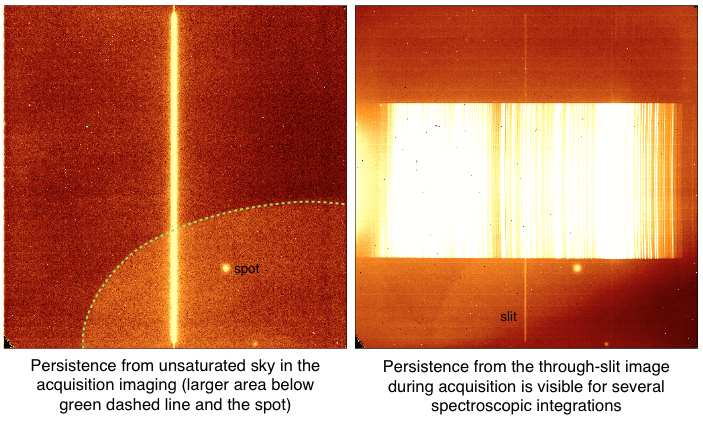
\includegraphics[width=0.6\textheight]{L2persistence.png}
  \caption[Persistence example]{Example for the persistence effect (Courtesy
    of LBT website\textsuperscript{\ref{fn:persistence}})}
  \label{fig:h2rg_persistence}
\end{figure}


However, since the determination of this pattern relies on observations previously done, this approach requires access to these data, which might arise from completely other observing runs and are therefore proprietary.
Therefore, the avoidance of persistence, i.e. a sophisticated planning / persistence management should be one of the major goals for the planning of the observations and the operational concept.
In case a persistence correction is required, a subtraction of a persistence map (\EXTCALIB{PERSISTENCE_MAP}) is foreseen in any individual recipe. This map is created by the recipe \REC{metis_det_persistence} (cf. Section~\ref{rec:metis_det_persistence}) , which is carried out by \ac{ESO} and relies on the algorithm provided by \ac{ESO}.

%\TODO{Will have access to a HDRL function from ESO.
%The interface is TBD.
%Subtraction of persistence image as determined by ESO.
%Need to reference ESO docs for this.
%How does the scaling happen?
%Is there an API endpoint for this?}


\subsection{Detector Masks}\label{ssec:criticaldetetctormasks}

In MATISSE the engineers created specific masks covering 32 pixels at the edge of the Aquarius detector, which was prone to crosstalk.
Crosstalk probably arises from the shared series buses in the detector readout electronics (see Figure on page 8 in~\cite{matisse_minutes}).
For the METIS detectors similar masks as in MATISSE are forseen in order to correct for crosstalk (cf. Polarion METIS-3093).
In~\cite{matisse_minutes}, the correction is described as follows:

\begin{displayquote}
    Cross-talk correction is done in two steps using the masked pixels in the vertical direction, which are equivalent to two masked outputs.
    \begin{itemize}
        \item Step 1 : The whole line is corrected by an offset.
        \item Step 2 : Each pixel is corrected using the corresponding masked pixel in terms of raw
            number in the two vertical masked outputs.
    \end{itemize}
\end{displayquote}

Fig.~\ref{fig:detmasks} taken from~\cite{matisse_minutes}, the minutes
of a detector meeting between the METIS and MATISSE consortia held in May 2017 in Bonn.
\begin{figure}[ht]
  \centering
  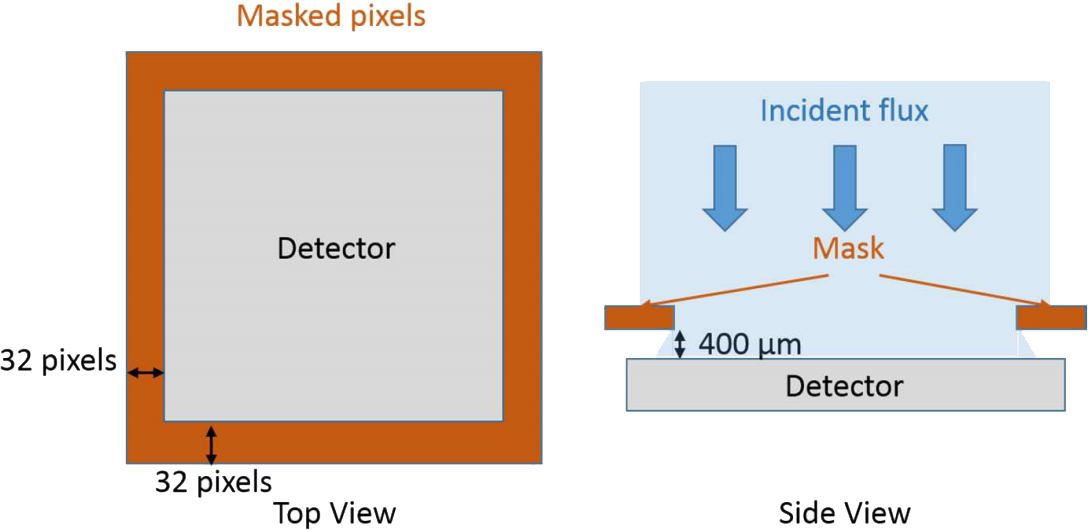
\includegraphics[width=0.6\textheight]{detmasks}
  \caption[Aquarius detector masks]{Aquarius detector masks as
    realised in MATISSE (\cite{matisse_minutes}, courtesy of
    S. Mouzali).}
  \label{fig:detmasks}
\end{figure}


%\begin{figure}[ht]
%  \centering
%  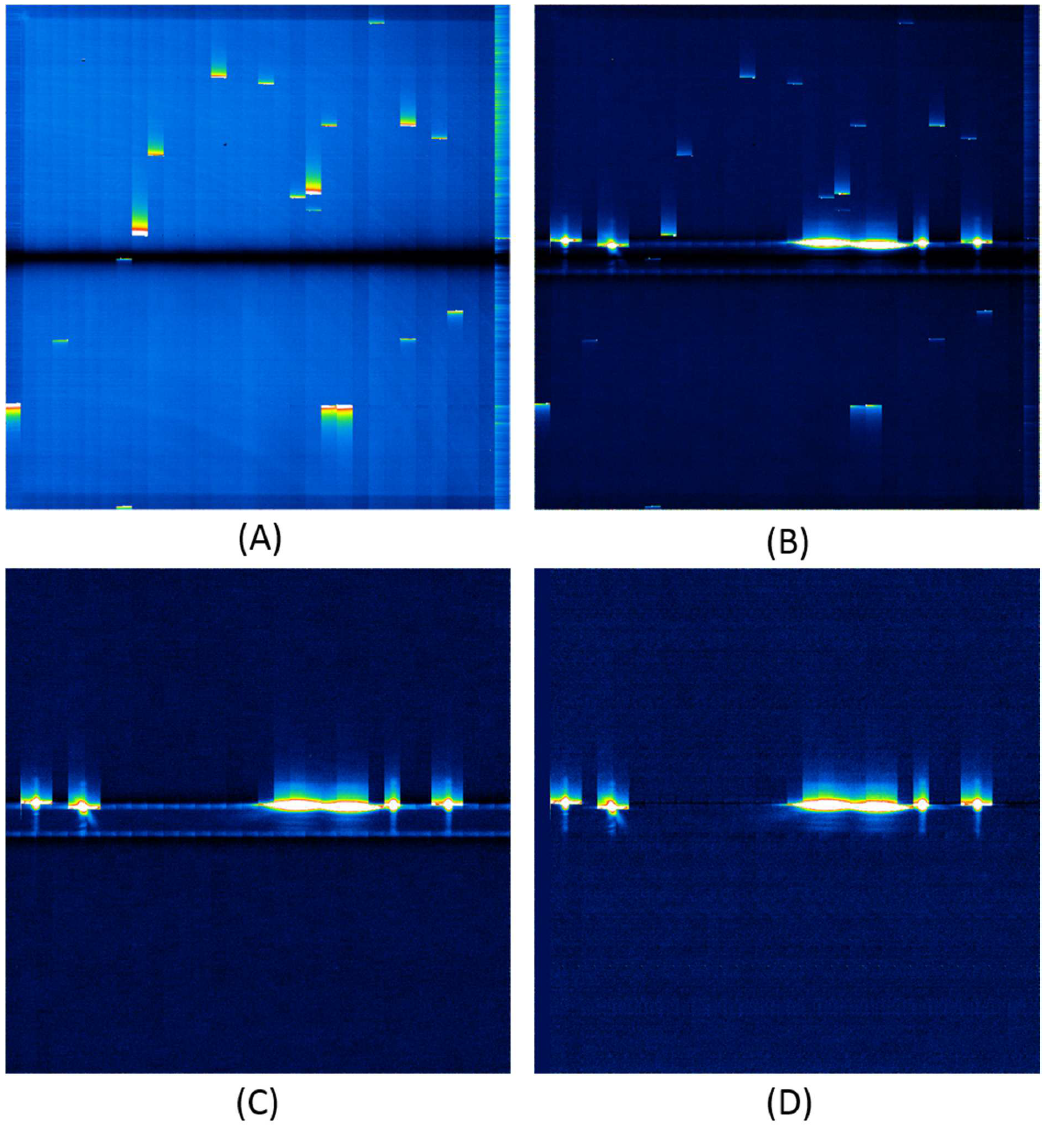
\includegraphics[width=0.4\textheight]{crosstalk.png}
%  \caption[Detector crosstalk]{Detector crosstalk example. See
%  \cite{matisse_minutes}
%    for an explanation.}
%  \label{fig:crosstalk}
%\end{figure}

\begin{figure}[ht]
  \centering
  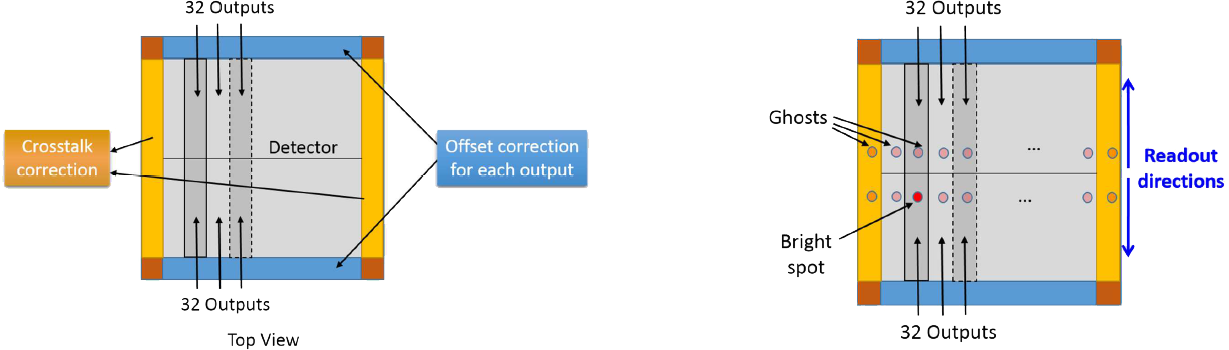
\includegraphics[width=0.6\textheight]{crosstalk2.png}
  \caption[Detector crosstalk correction]{Correction for the crosstalk
    (\cite{matisse_minutes}, courtesy of S. Mouzali).}
  \label{fig:crosstalk2}
\end{figure}

MATISSE has dealt with the detector masks adequately and the same procedures will be used for METIS; a prototype is therefore not made.

% \TODO{
%     Look into the MATISSE docs as to how this was done
%     Delivers a bias/dark/ron value?
% }

\subsection{Bad pixel determination}\label{ssec:criticalbadpixeldetermination}

Bad pixels are an issue in any detector and have to be monitored and stored.
This is usually done with the help of DARK and FLATFIELD frames.
Cold/hot pixels can be identified by using DARKS since they have pixel values which are far from an expected values (e.g.\ median value).
Non-linear pixels can be detected with illumination flats, that is, the detector is illuminated uniformly by a flatfield source.
Using several exposure times / flux levels, non-linearities in pixels can be found by fitting polynomials to each individual pixel.

Each processed data product will contain a data quality extension for each
data extension (Section~\ref{sssec:processeddataextensions}), including
calibration data products.
Note that every science product will need its own bad pixel map, to keep track
of pixels affected by persistence.
Having an extra data quality extension will therefore not significantly affect
the data volume.

It is therefore not necessary to have a dedicated data product for the
bad pixels;
the propagation of bad pixels through the pipeline can be done
by copying (XOR-ing) the bits of the data quality layer of the calibration data
into the data quality layer of the data that is being processed.
Nevertheless, it can be useful to have such a data product, and several recipes
can therefore have a \PROD{BADPIX_MAP_det} as output or input anyway.

We will use a bad pixel classification similar to the convention introduced in
the X-Shooter Pipeline Manual (cf.\ Section 11.3 in~\cite{xshooter_manual}),
adapted to our needs.


%\TODO{
%    Surely every other instrument on planet earth has some sort of algo for this.
%    Need to determine the format of the bad pixel mask (bool?)
%    Take XSHOOTER as example ftp://ftp.eso.org/pub/dfs/pipelines/xshooter/xshoo-pipeline-manual-12.19.1.pdf
%}

\subsection{Background subtraction}\label{ssec:criticalbackgroundsubtraction}
Observations in the mid-infrared are affected by the high sky background, the telescope background, and detector variations and non-linearities.
A proper background correction is thus essential to ensure accurate photometric and spectroscopic analysis of the observed sources.
As METIS will face an unprecedented level of complexity in the background subtraction due to
\begin{enumerate}
    \item the high background dominated by the large number of warm mirrors,
    \item the internal chopping, and
    \item the complexities of nodding with an AO-corrected instrument,\end{enumerate}
a dedicated research project has been started to better understand the origin of chop-residuals and to evaluate chop-only background removal strategies.


% Hence, the dedicated pipeline algorithms will ultimately depend on the chosen strategy for each METIS detector, e.g.\ dithering, classical chop-nod, chop-counter-chop (in 1D or 2D), drift scanning.
%This is particularly relevant for the N bands where, for instance, the instability of the AQUARIUS detector response demands chopping at much higher frequencies.
% More details on dedicated research project and the proposed strategies are given in the Calibration Plan~\cite{METIS-calibration_plan} which serves as the base for the following.

Nevertheless, standard subtraction techniques (dithering, chopping and nodding)
will be used, which not require prototying. More complex algorithms that would
have required prototyping, e.g. involving principal component analysis, have been
ruled out since \ac{PDR}.

% \TODO{
%     N-band: Standard chop and nod using telescope chopper and internal nodder. See VISIR pipeline.
% }

\subsubsection{LM bands}
Small ($< 5 \arcsec$) and slow (1 min timescale) dithered offsets of the field with respect to the LM IMG or \ac{IFU} detector are expected to be performed by the METIS-internal chopper mirror.
The pipeline will determine the sky background from the dithered images and produce background maps without the sources and background-subtracted versions of the maps with the sources.
For In-field-dithering, this is done by determining a flux scaling factor for each ``dither'' position, aligning the exposures (by either using a 2d cross-correlation routine on bright sources or by using the offset values applied to the chopper), scaling the frames to a common median and removing objects by rejecting the highest and lowest pixels.
The remaining pixels are then averaged, or medianed, to produce the sky frame which is then scaled to match the median of the object frame before being subtracted.
The sky subtraction is further improved by following the previous steps to produce the combined image to locate all the sources.
Then the background frames are combined again while excluding the sources positions.
The best approach to determine the flux scaling factor of each dither exposure is yet to be determined (e.g.\ by median scaling or by a 2D/PCA approach based on~\cite{Hunziker2018}).
The pipeline would also support sky subtraction using separate sky images for out-of-field dithering modes, i.e.\ when the observed field is crowded or full of extended emission.

\subsubsection{N bands}\label{sssec:nbandsbackgroundsubtracion}
To ensure proper background sampling at the longer wavelengths, small ($< 5 \arcsec$) and fast ($\approx 10 \mathrm{Hz}$) chopping offsets of the field with respect to the N IMG detector are expected to be performed by the METIS-internal chopper mirror.
The chopping residuals from the previous step will be corrected by nodding the telescope to a different position and repeating the same chopping procedure.
%The chopping and nodding sequence is expected to follow what is currently being done with VISIR.
A 3-point parallel nodding sequence is followed, which should give a higher \ac{SNR} than the 2 point pattern used in e.g.~VISIR (cf.~\cite{METIS-operational_concept}).

The pipeline will determine the sky background from the chopped and nodded images and produce background maps without the sources and background-subtracted versions of the maps with the sources.
For each nodding cycle the subsequent chop-cycle frames are subtracted from each other (mean of on-source frames minus mean of off-source frames) resulting in a single chop-difference frame, i.e. nod half-cycle frame.
Then for subsequent nodding cycles the nod half-cycle frames are subtracted from each other resulting in a nod-difference frame.
The mean of all nod-difference frames is the final background-subtracted image.
Additionally, the optimal extraction (PSF-weighting) will be used to subtract the positive/negative source images from the final background-subtract image (2/3/4 depending on the relative chopping/nodding directions) to produce a single stacked image of the sources of interest.

There might be extensive spatial modulation (dithering) within a nod half cycle.
That is, the 3-point chop pattern is repeated a few times, then the slightly move the central position is moved slightly after which the 3-point chop pattern is repeated.
This is done several times in a nod-half cycle, and then repeated in the same pattern in the other nod position after the nod is performed.
This is to mitigate the (many) bad/hot pixels in the GeoSnap array, therefore chop-cycle frames will be subtracted such that the bad pixels can be worked around.

\subsection{Wavelength calibration and distortion correction}\label{ssec:criticalwavelengthanddistortion}
The wavelength calibration and distortion correction critical algorithm is split in a LSS part (Section~\ref{ssec:criticalwavelengthanddistortionlss}) and an IFU part (Section~\ref{ssec:criticalwavelengthanddistortionifu}).

\subsubsection{LSS Wavelength calibration and distortion correction}\label{ssec:criticalwavelengthanddistortionlss}
\newcommand{\pyred}{\textsc{PyReduce}}
\newcommand{\met}{\ac{METIS}}
\newcommand{\mir}{\ac{MIR}}
\newcommand{\lss}{\ac{LSS}}
\newcommand{\elt}{\ac{ELT}}
\newcommand{\scope}{\textsc{ScopeSim}}

% The goal of this calibration step is to create rectified 2D orders with the spatial coordinate along the slit and the calibrated wavelength coordinate along the dispersion direction. This can be achieved in three steps:

The \mir~range is dominated by thermal and line emission in the Earth's atmosphere. These emission lines can be used to determine both the curvature/tilt-distortion of the LSS spectrograph and subsequently the wavelength calibration. We adapt the \pyred~package \cite{pis21} employing state-of-the-art functions for optimal extraction of echelle spectra.  The package works successfully on several ESO instruments and has been adopted for the CRIRES+ pipeline. In the following sections we assess its functionality on simulated \met~ spectroscopic data.


\subsubsection{Implementing METIS in \pyred}\label{sec:pyred_mic}
% \todo[inline]{TODO-NS: to be edited}
\pyred~\cite{pis21} is an  open source Python implementation\footnote{\url{https://github.com/AWehrhahn/PyReduce}} (with some C components)  of the IDL-based REDUCE pipeline \cite{pis02}.  The package supports data reduction of several echelle spectrographs, e.g. CRIRES+,  HARPS, and can be optimized to work on any instrument, also on a  long slit spectrograph as in the case of \met. In order to adapt \pyred~to work on simulated \met~\lss~data, we created a custom instrument class  and defined all the needed parameters to run \pyred~within a single script (Method~1\footnote{\url{https://pyreduce-astro.readthedocs.io/en/latest/instruments.html}}). This provided a quick way to finding the needed settings to  run the package successfully on \met~data before a complete implementation is done following Method~2. The full implementation requires several configuration files: 
\begin{itemize}
\item Custom instrument class (\texttt{metis.py}) serving several functions such as loading a json file (\texttt{load\_info}) with FITS header information, finding  and sorting files (\texttt{sort\_files}) for the different reduction steps, modifying fits header information (\texttt{add\_header\_info}), finding the wavelength calibration guess file (\texttt{get\_wavecal\_filename}) etc.
\item Header keyword map (\texttt{metis.json})
\item \pyred~runtime configuration file (\texttt{settings\_metis.json}) 
\item Wavelength calibration initial guess  file (e.g. \texttt{metis\_lss\_m\_2D.npz}) containing a numpy recarray called \texttt{cs\_lines} which includes information on the detector positions of the wavelength calibration lines.
 % and their respective echelle orders. 
 More details in Sect.~\ref{sec:critalg_wavecal}
\item \pyred~runtime script (\texttt{metis\_example.py}), in which the user defines where the data are located, which \met~\lss~mode to use ($L$, $M$, or $N$-band), \pyred~steps to run, and where they could change any parameter pertaining to \pyred~steps before inserting them into the file \texttt{settings\_metis.json}.
\end{itemize}

Placing the above files in their respective \pyred~folders enables \pyred~to run \met~\scope~simulated files as any other instrument. \pyred~ performs many functions when reducing spectroscopic data  including basic data reduction like bias determination, flatfielding, continuum fitting. Here we investigate mainly the steps relevant to the mentioned critical algorithms: \texttt{"curvature", and "wavecal"}.
%-----------
\paragraph{Simulated input `raw' data}
To demonstrate the feasibility of adopting \pyred~algorithms to \metis~purposes we use data simulated with \scope~for all three \lss~modes ($L$, $M$, or $N$-band) for the $8000~\textrm{mas} \times 19~\textrm{mas}$ slit (see Fig.~\ref{fig:lmn_layout}). 
% \todo Details on the simulated data and the input files and settings used to generate them are listed in the DRLVT \cite{drlvt}. 
Then header keywords of the simulated data were added/modified to enable \pyred~to sort the individual files according to \texttt{metis.json}. Here we list the files - listed here for the case of $L$-band but similaily to $M$ and $N$-bands - that are used to operate \pyred, which can be downloaded from\footnote{\url{https://www.dropbox.com/sh/h1dz80vsw4lwoel/AAAqJD_FGDGC-t12wgnPXVR8a?dl=0}}: 
\begin{itemize}
   \item \texttt{lss\_l\_thermal.fits}: spectroscopic flat field (Fig.~\ref{fig:ff})
   \item \texttt{lss\_l\_pinholes.fits}: pinhole frame with the flat field (Fig.~\ref{fig:pinh})
   \item \texttt{lss\_l\_sky.fits}: sky emission line spectrum covering the full slit (Fig.~\ref{fig:sky})
   \item \texttt{lss\_l\_star.fits}: star spectrum ("science" target) (Fig.~\ref{fig:star})
\end{itemize}

\begin{figure}[!h]
  \centering
  \includegraphics[width=\textwidth]{figures/LSS_CrtAlg_files/{METIS_LSS_SpectralLayout_px}.png}
  \caption{\textbf{Spectral layout of the METIS LSS mode of all three supported bands}: The spectral layout is shown here for all three \lss~bands as taken from the corresponding trace files - after transforming from mm to px coordinates- from the \met~IRDB for a slit length of 8 arcsec.}
  % \caption{\textbf{Spectral layout of the METIS LSS mode of all three supported bands}: The spectral layout is shown here for all three \met~\lss~bands where sky emission lines fall on them. }

  \label{fig:lmn_layout}
\end{figure}

\begin{figure}[!h]
\centering
  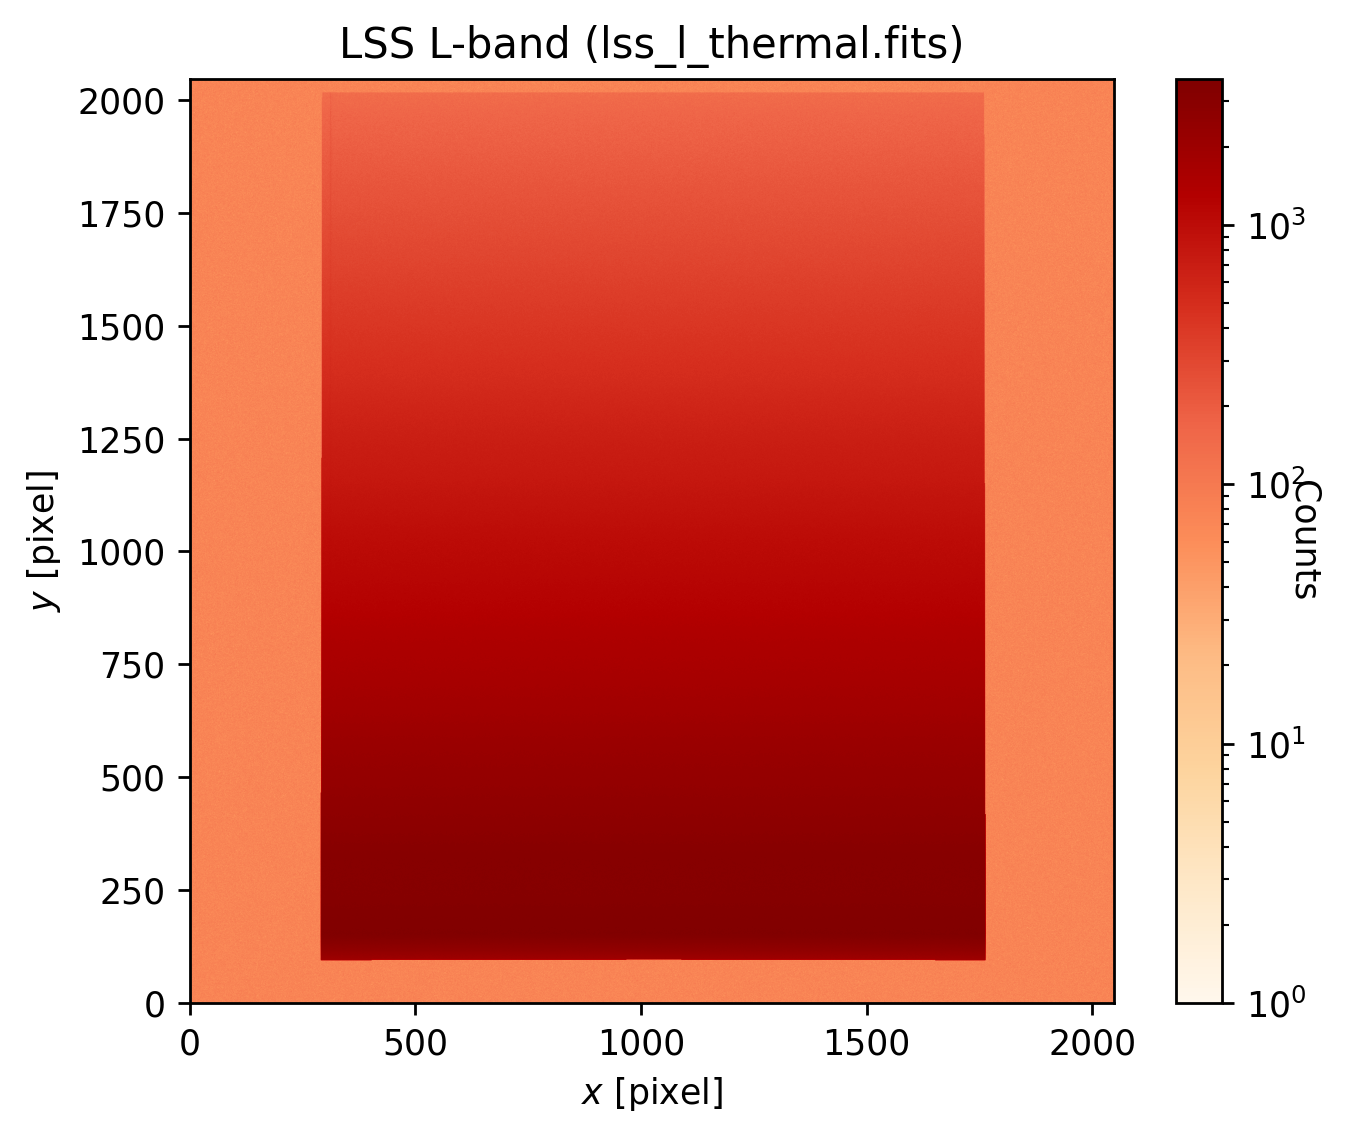
\includegraphics[height=4cm,keepaspectratio]{figures/LSS_CrtAlg_files/lss_l_thermal.fits.png}
  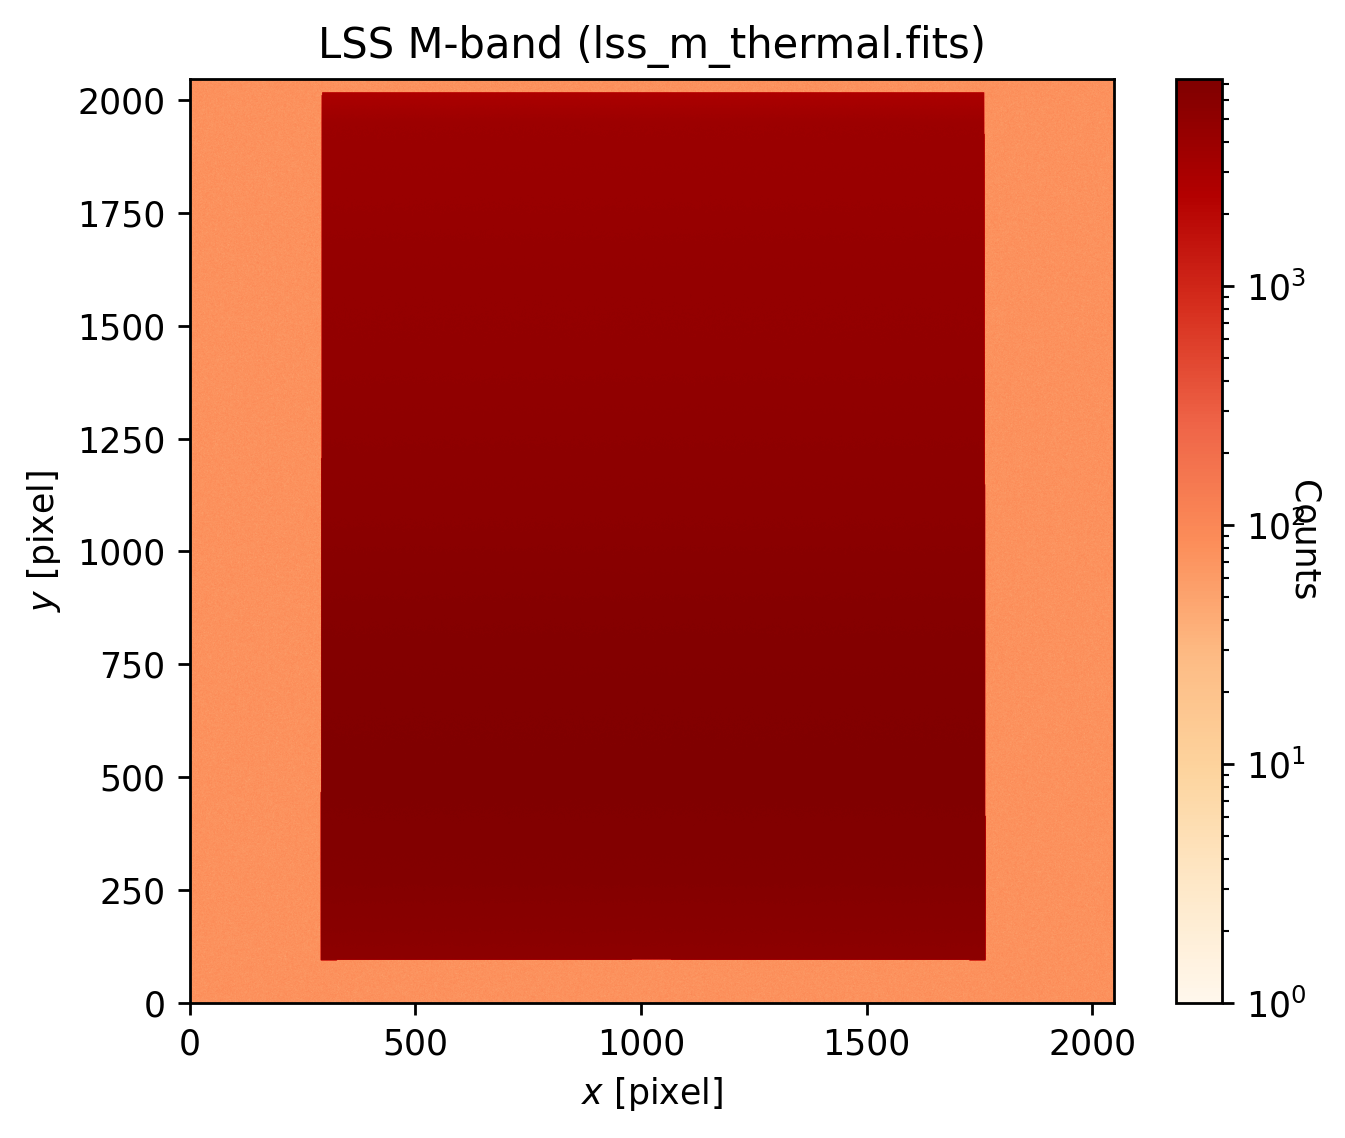
\includegraphics[height=4cm,keepaspectratio]{figures/LSS_CrtAlg_files/lss_m_thermal.fits.png}
  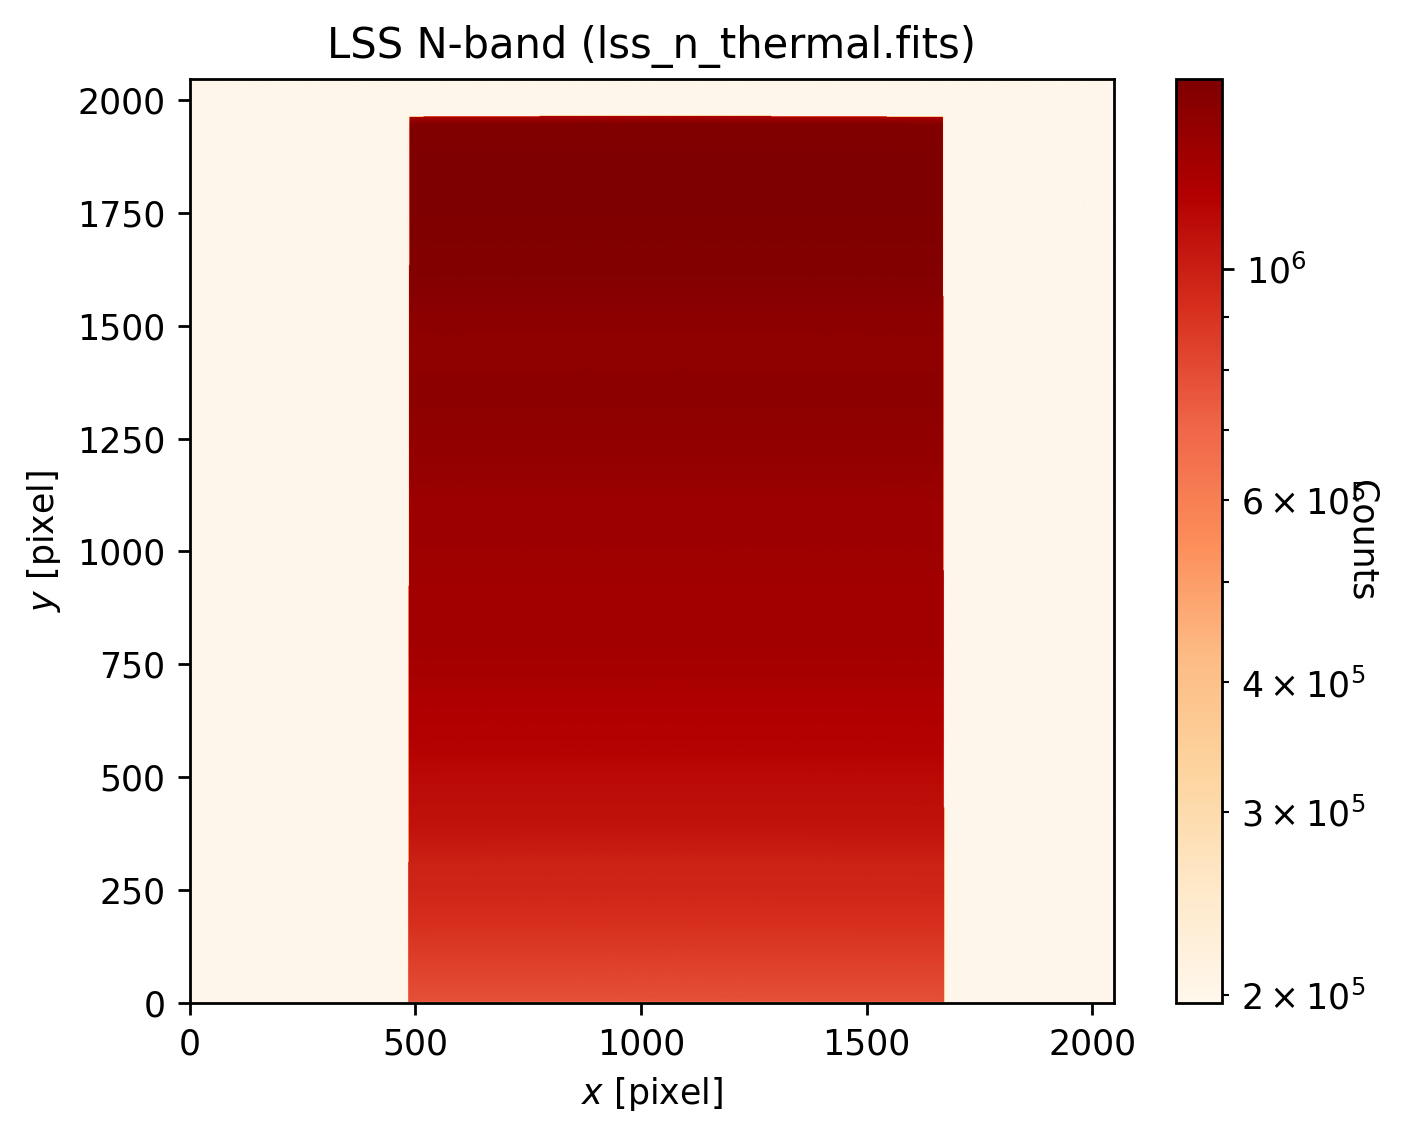
\includegraphics[height=4cm,keepaspectratio]{figures/LSS_CrtAlg_files/lss_n_thermal.fits.png}
  \caption{Long-slit spectroscopic flat field frames for \lss~$L$-, $M$-, and $N$-bands.} 
  \label{fig:ff}
\end{figure}

\begin{figure}[!h]
\centering
  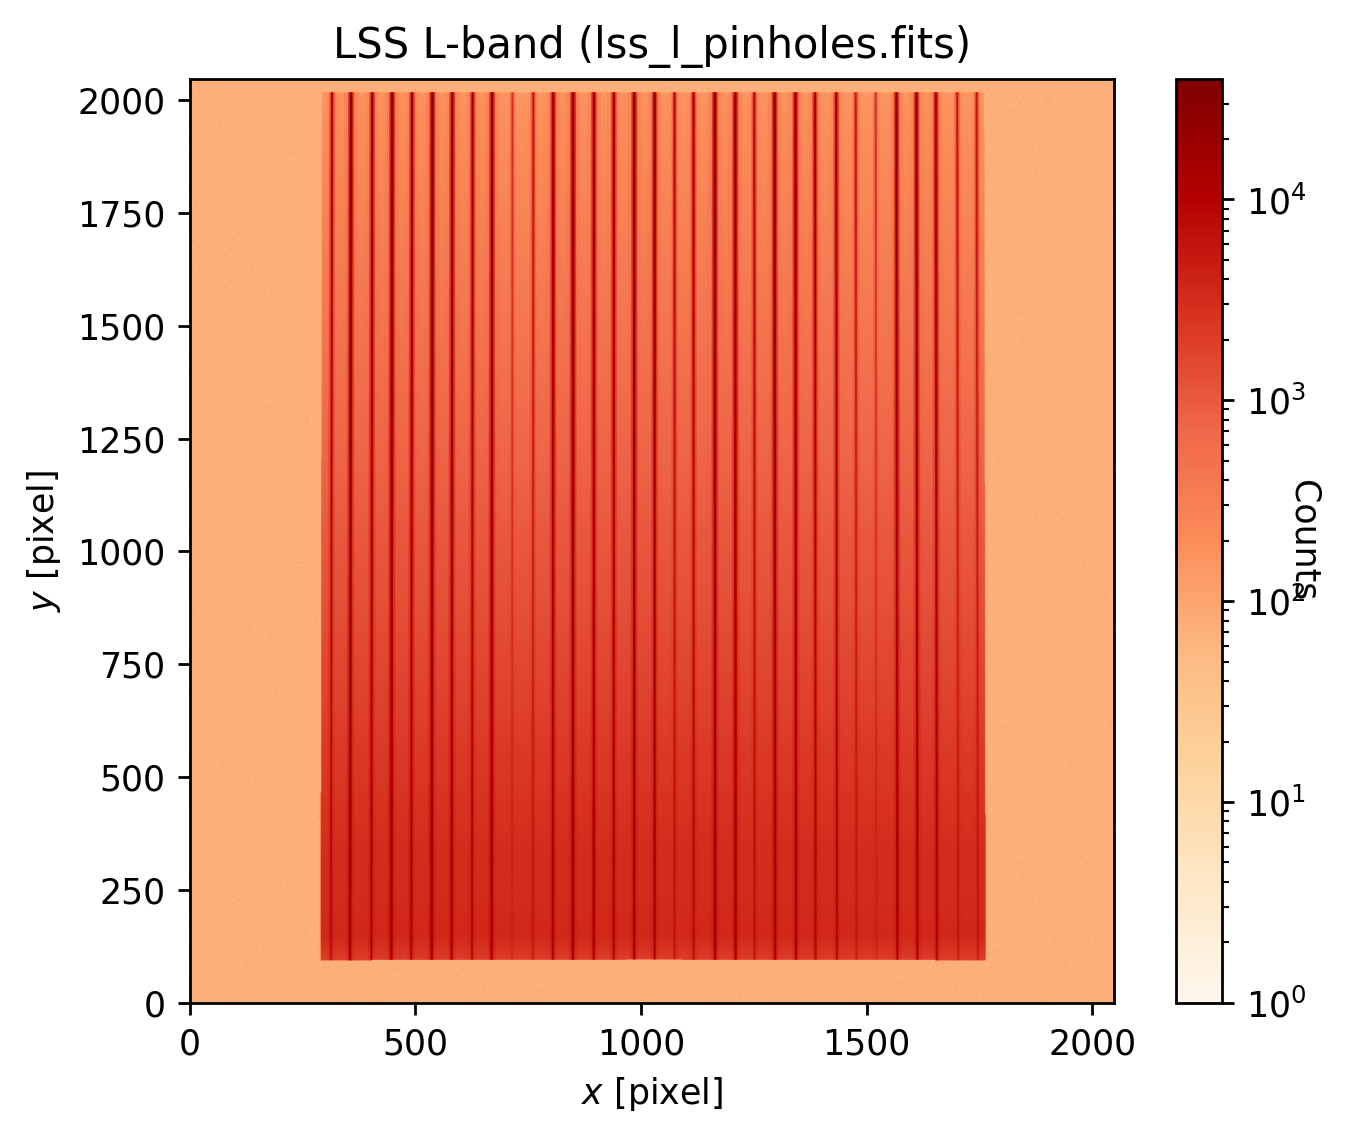
\includegraphics[height=4cm,keepaspectratio]{figures/LSS_CrtAlg_files/lss_l_pinholes.fits.png}
  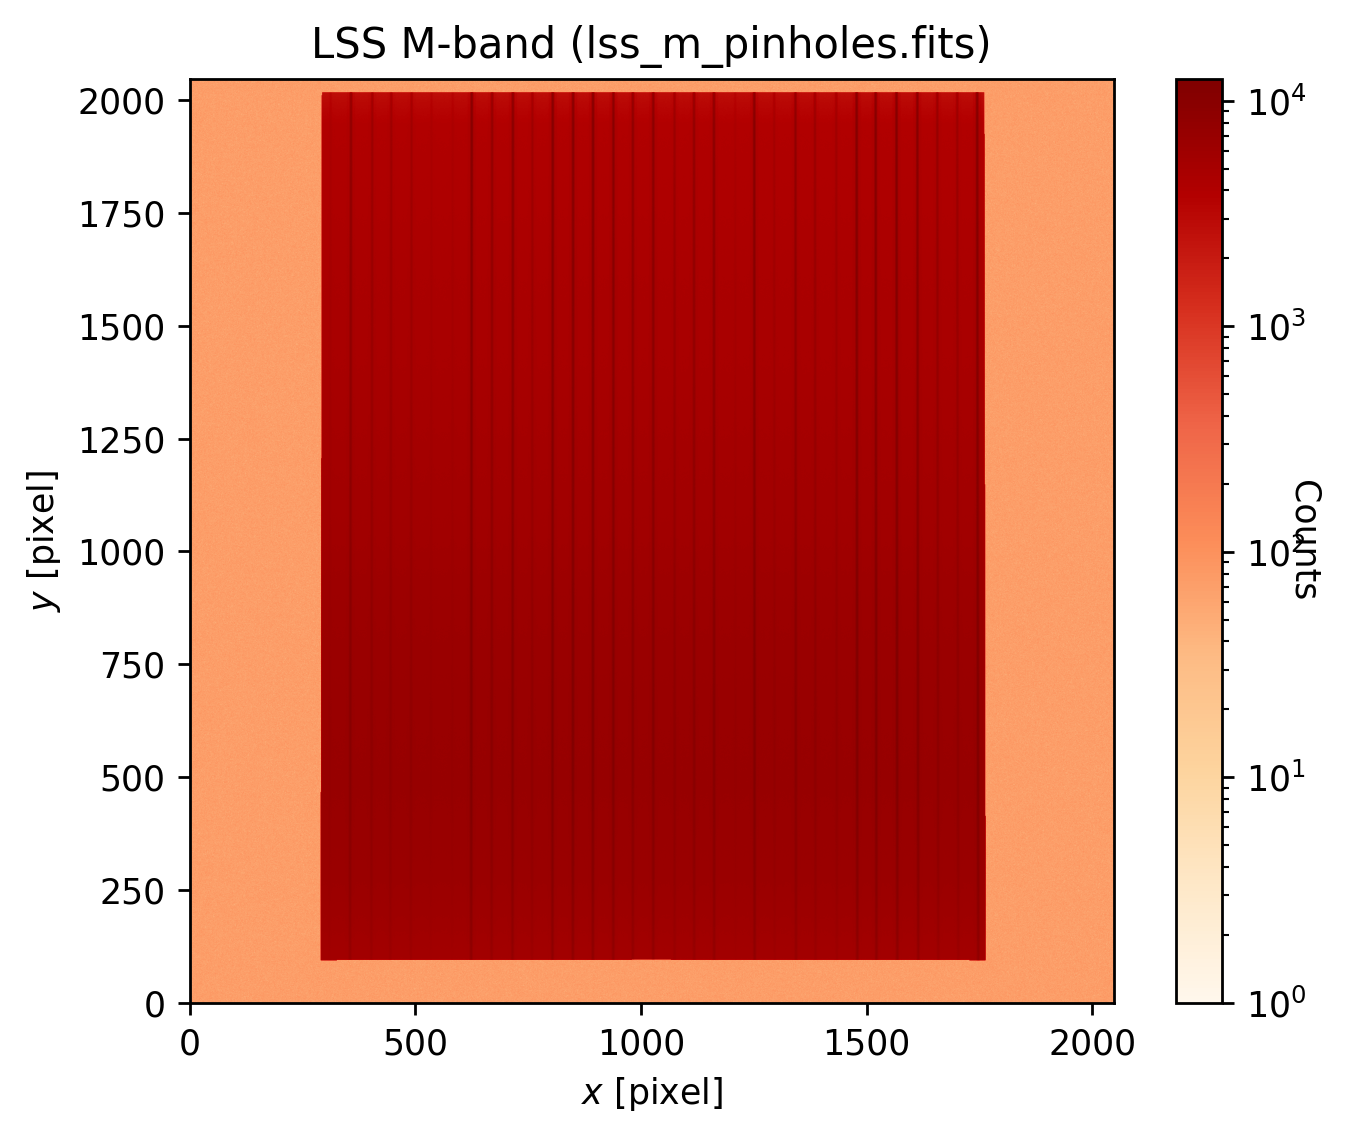
\includegraphics[height=4cm,keepaspectratio]{figures/LSS_CrtAlg_files/lss_m_pinholes.fits.png}
  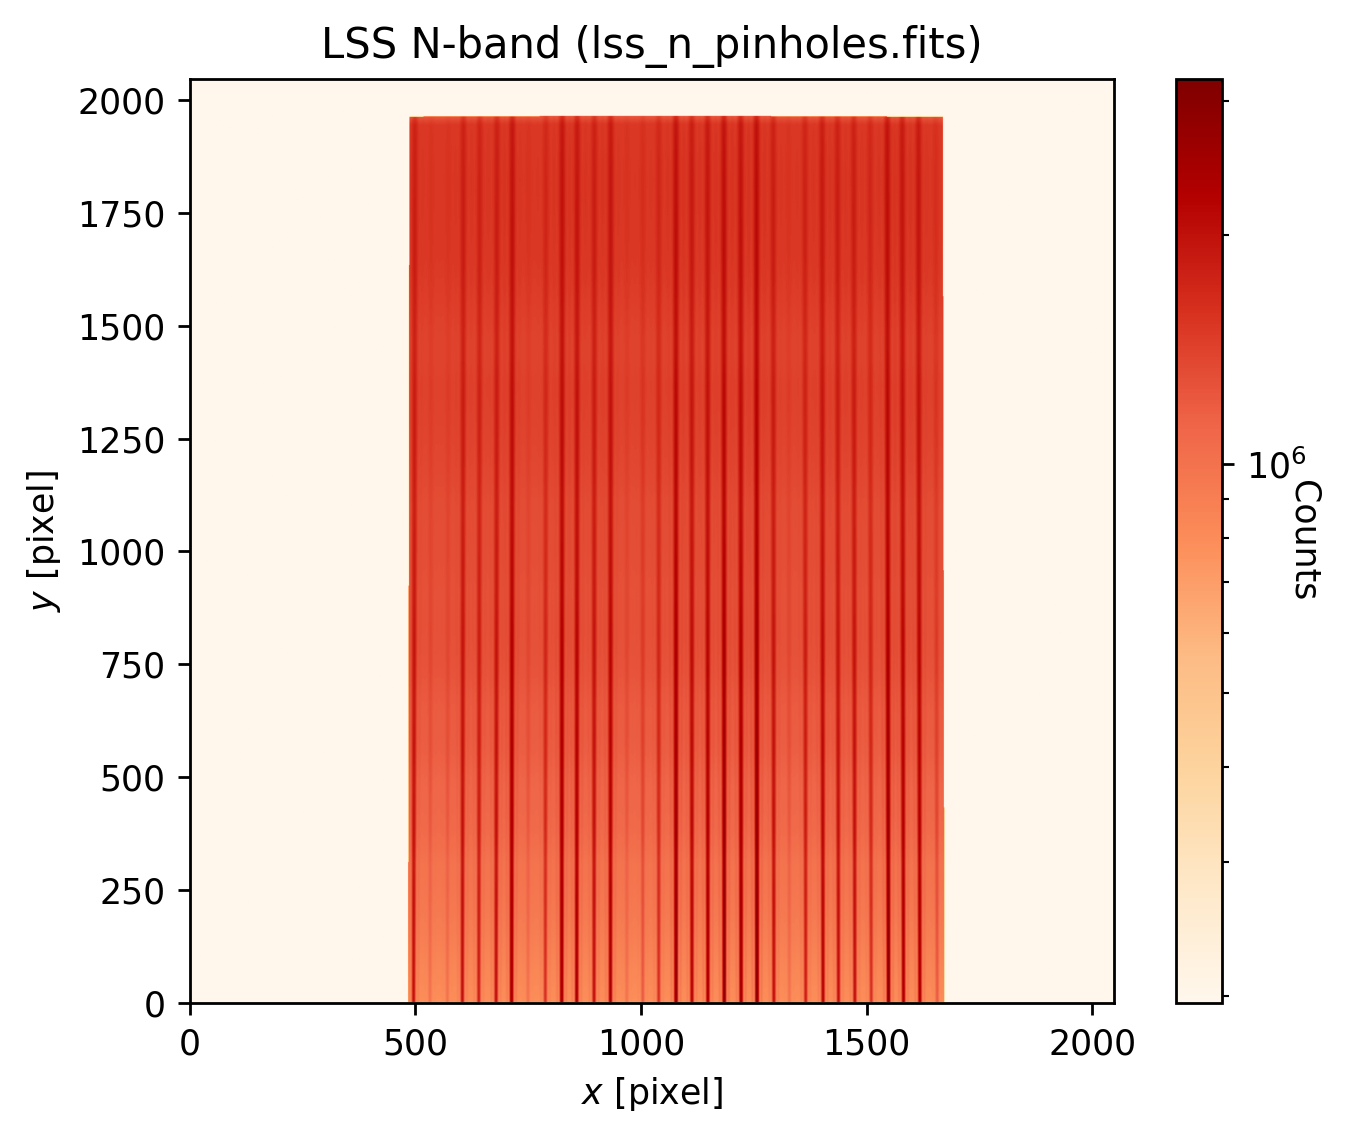
\includegraphics[height=4cm,keepaspectratio]{figures/LSS_CrtAlg_files/lss_n_pinholes.fits.png}
  \caption{Pinholes with the flat field frames for \lss~$L$-, $M$-, and $N$-bands.} 
  \label{fig:pinh}
\end{figure}

\begin{figure}[!h]
\centering
  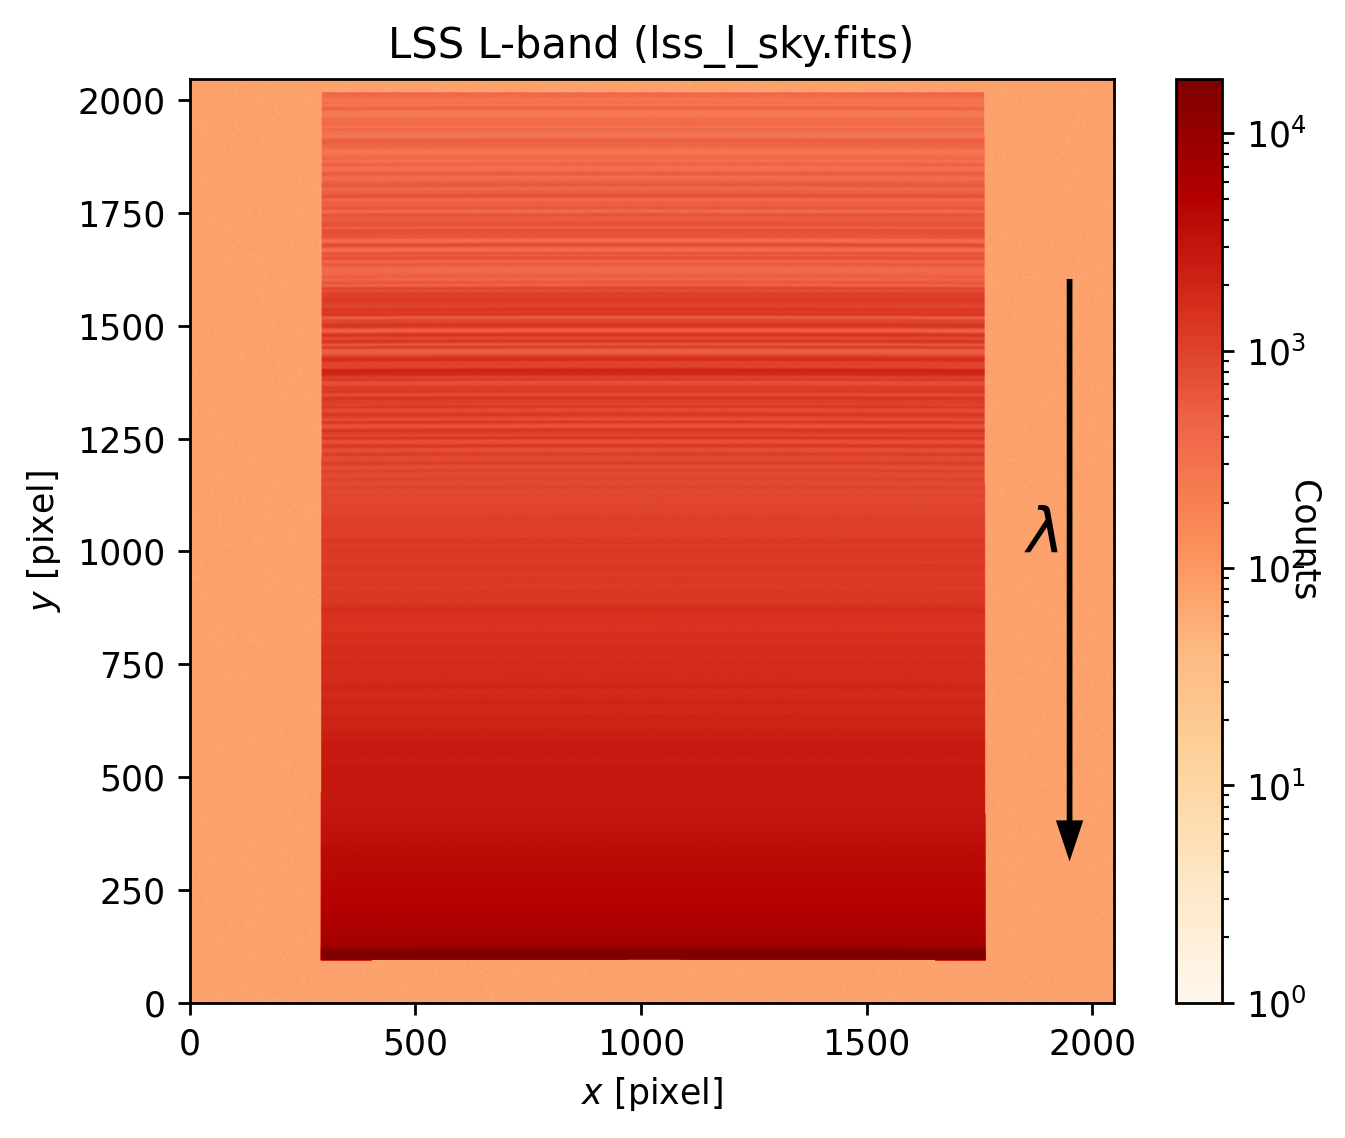
\includegraphics[height=4cm,keepaspectratio]{figures/LSS_CrtAlg_files/lss_l_sky.fits.png}
  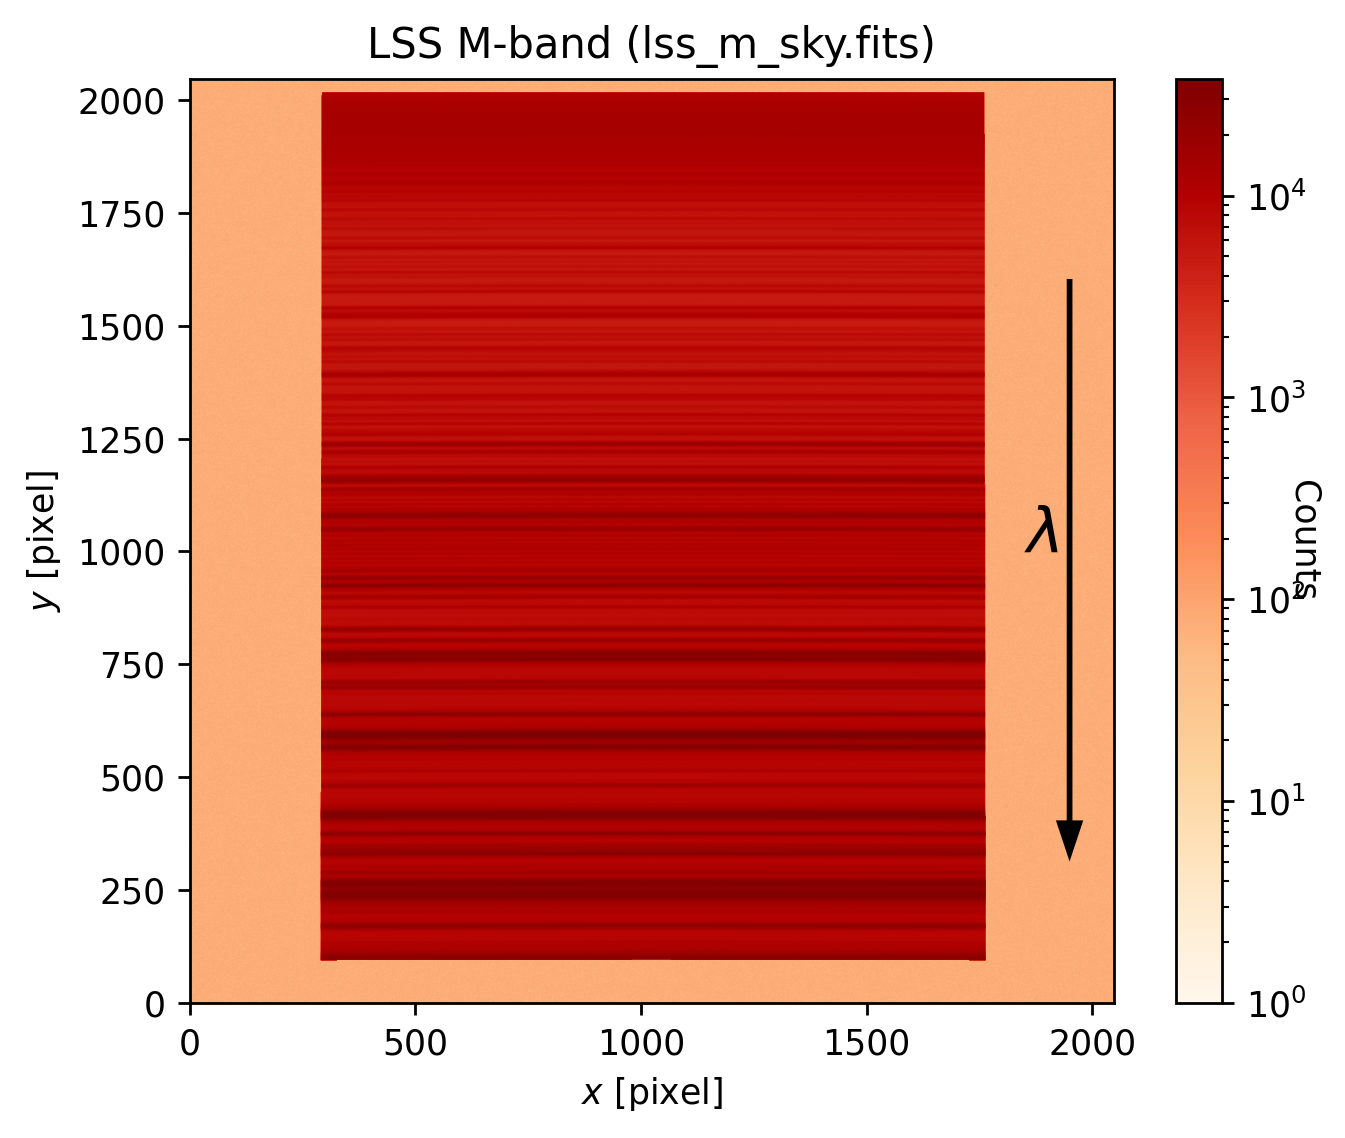
\includegraphics[height=4cm,keepaspectratio]{figures/LSS_CrtAlg_files/lss_m_sky.fits.png}
  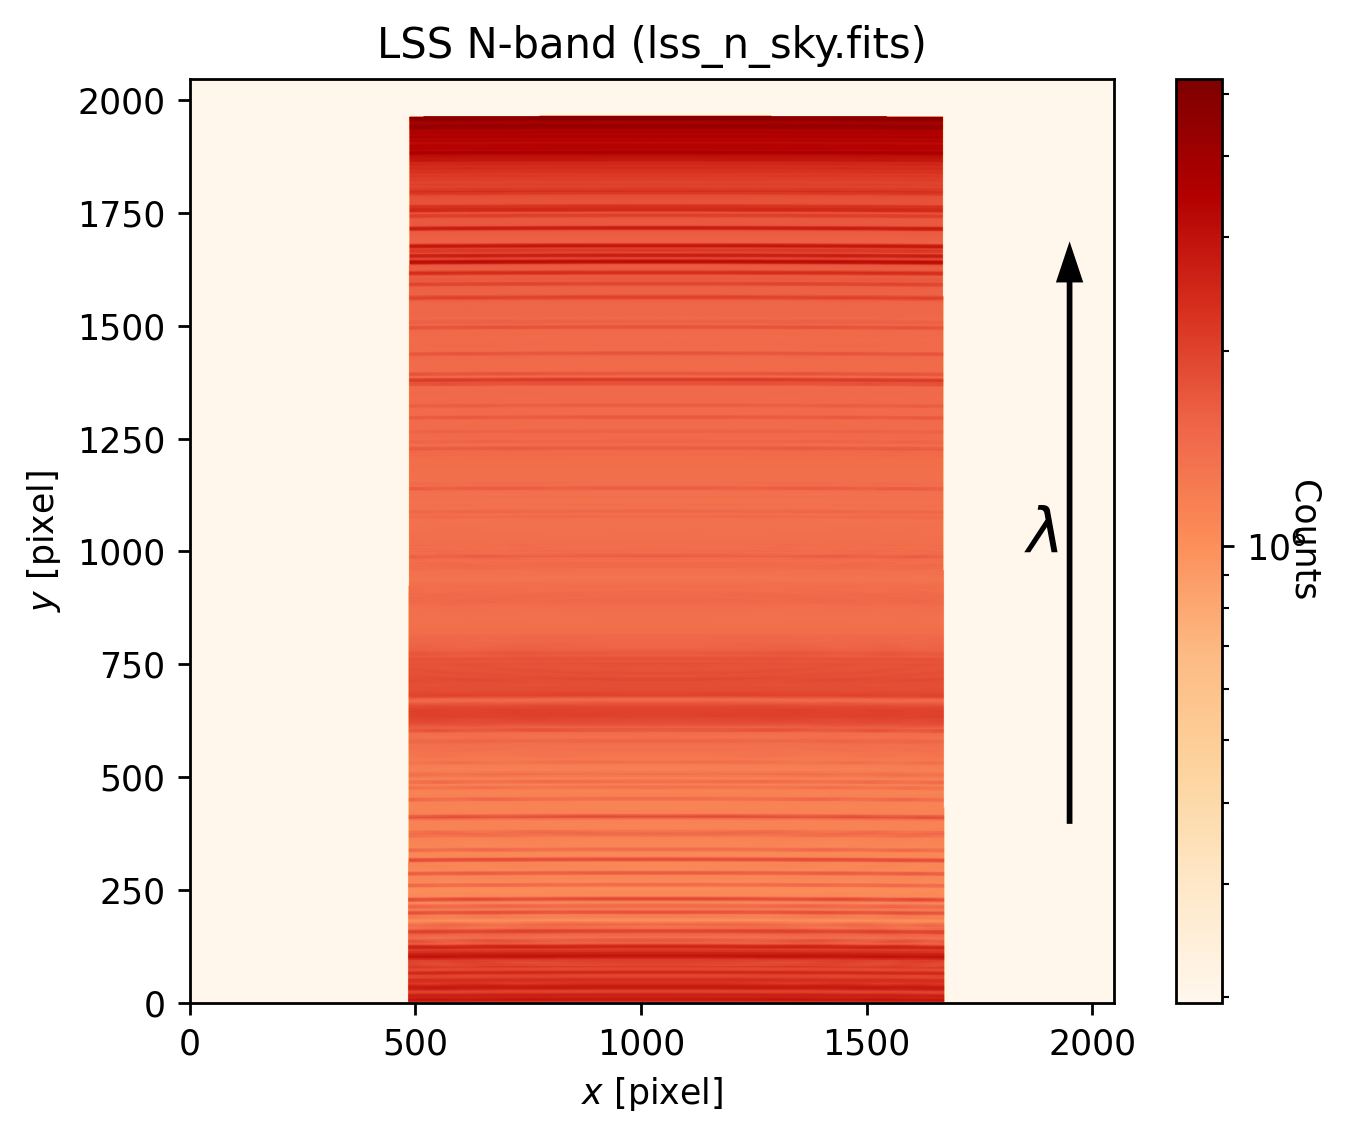
\includegraphics[height=4cm,keepaspectratio]{figures/LSS_CrtAlg_files/lss_n_sky.fits.png}
  \caption{Sky emission line spectrum frames for \lss~$L$-, $M$-, and $N$-bands.} 
  \label{fig:sky}
\end{figure}


\begin{figure}[!h]
\centering
  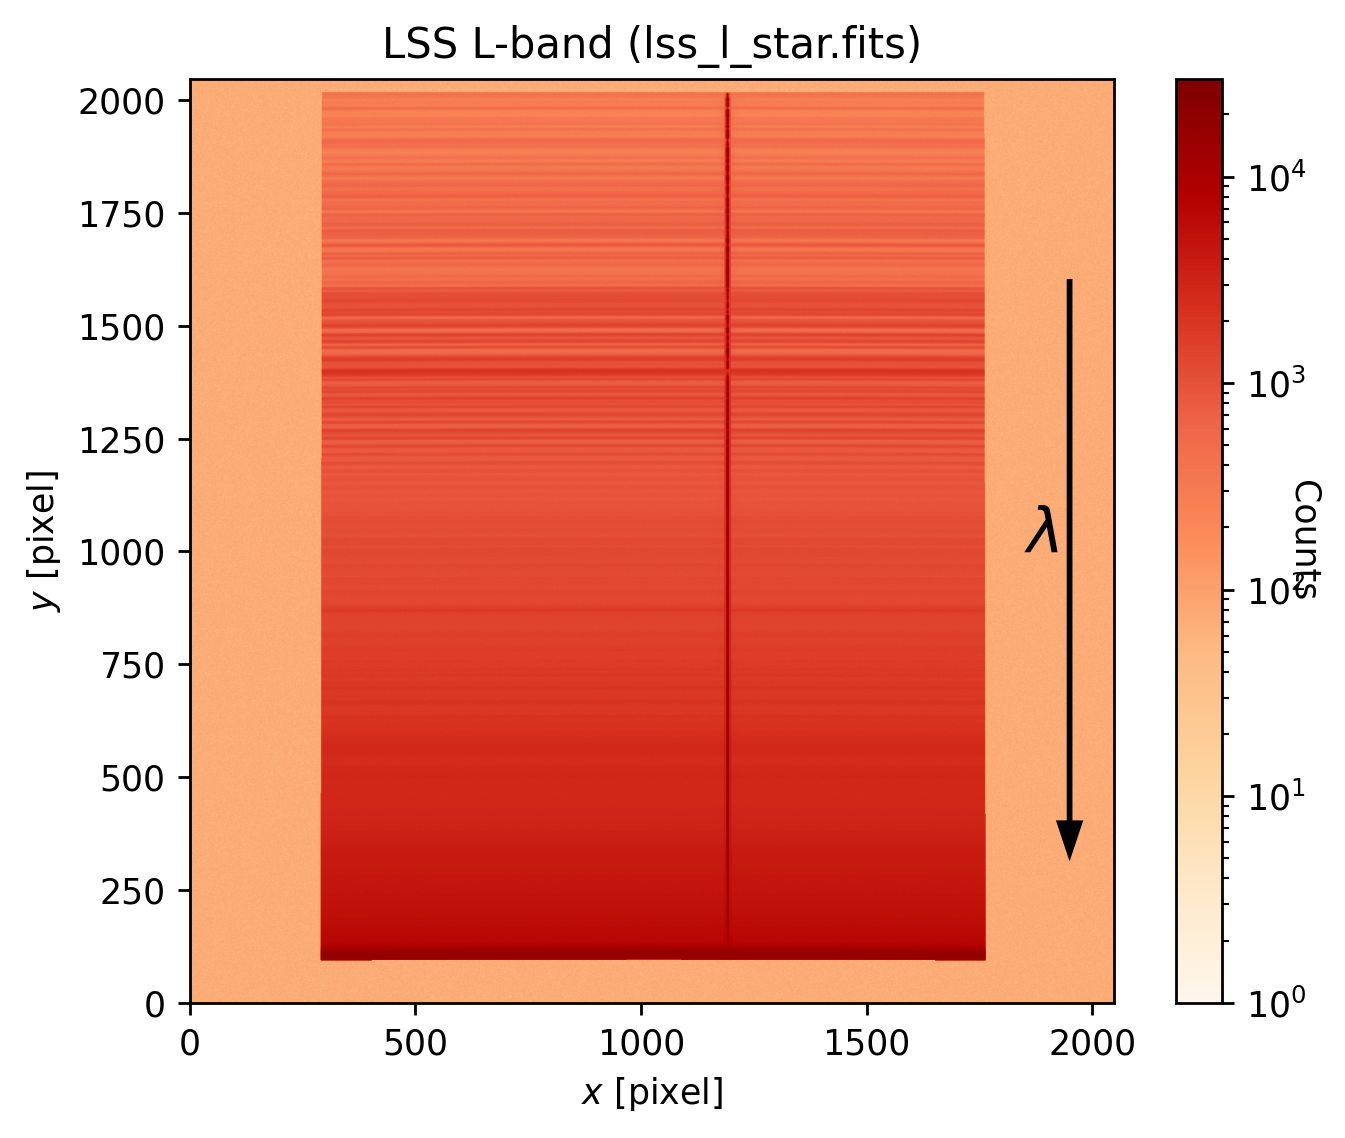
\includegraphics[height=4cm,keepaspectratio]{figures/LSS_CrtAlg_files/lss_l_star.fits.png}
  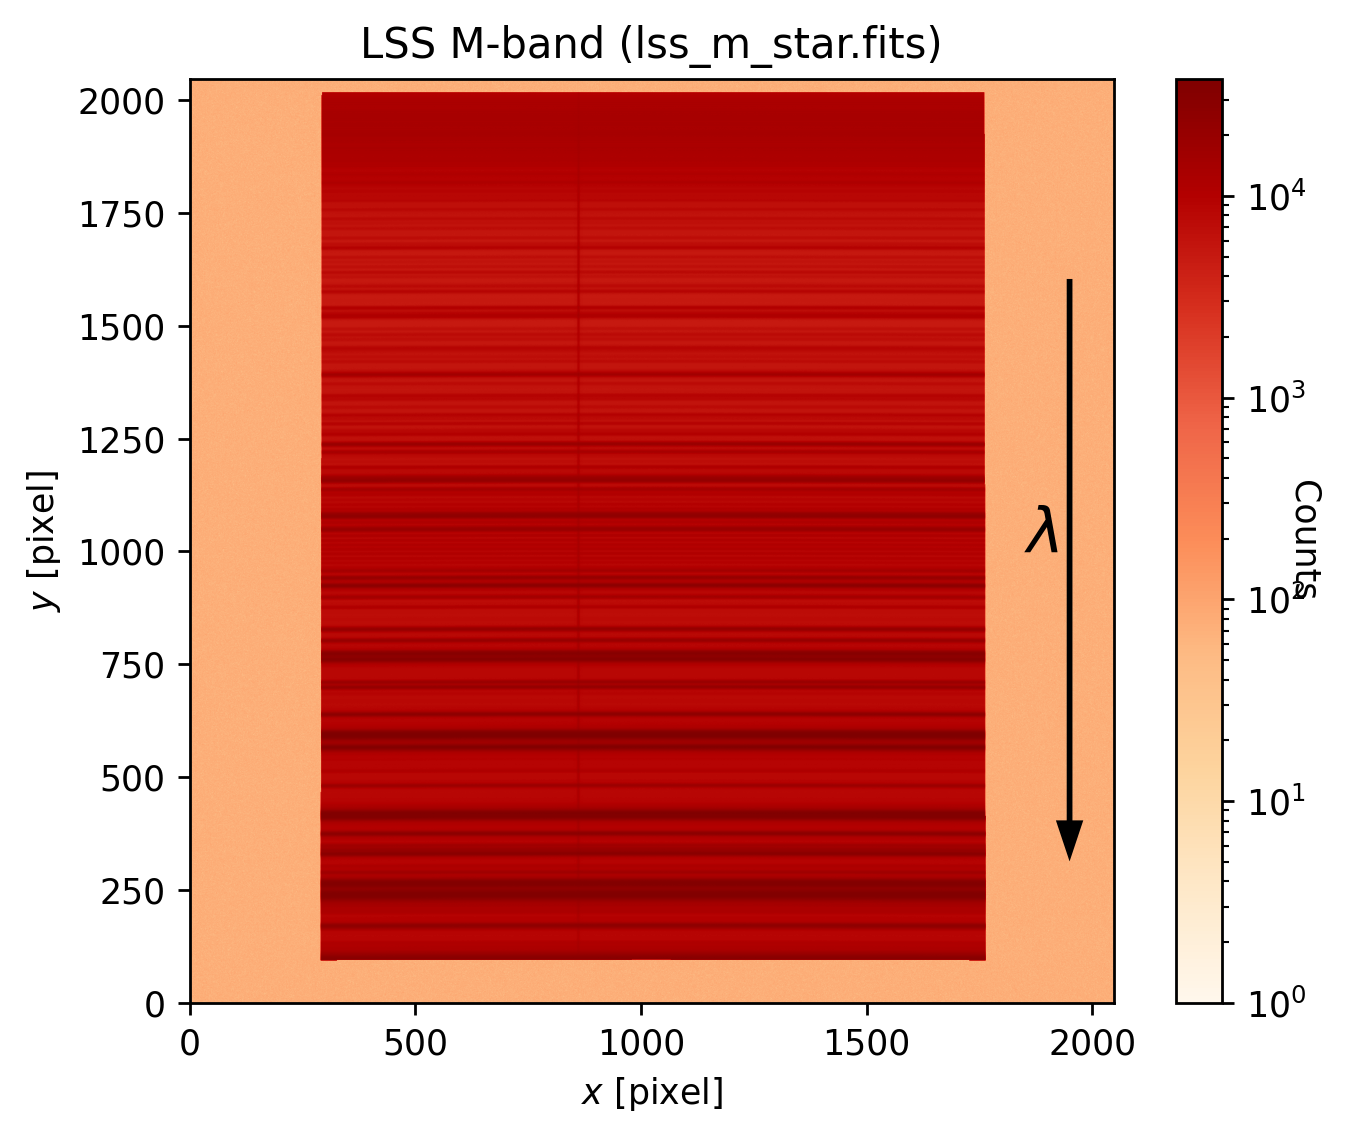
\includegraphics[height=4cm,keepaspectratio]{figures/LSS_CrtAlg_files/lss_m_star.fits.png}
  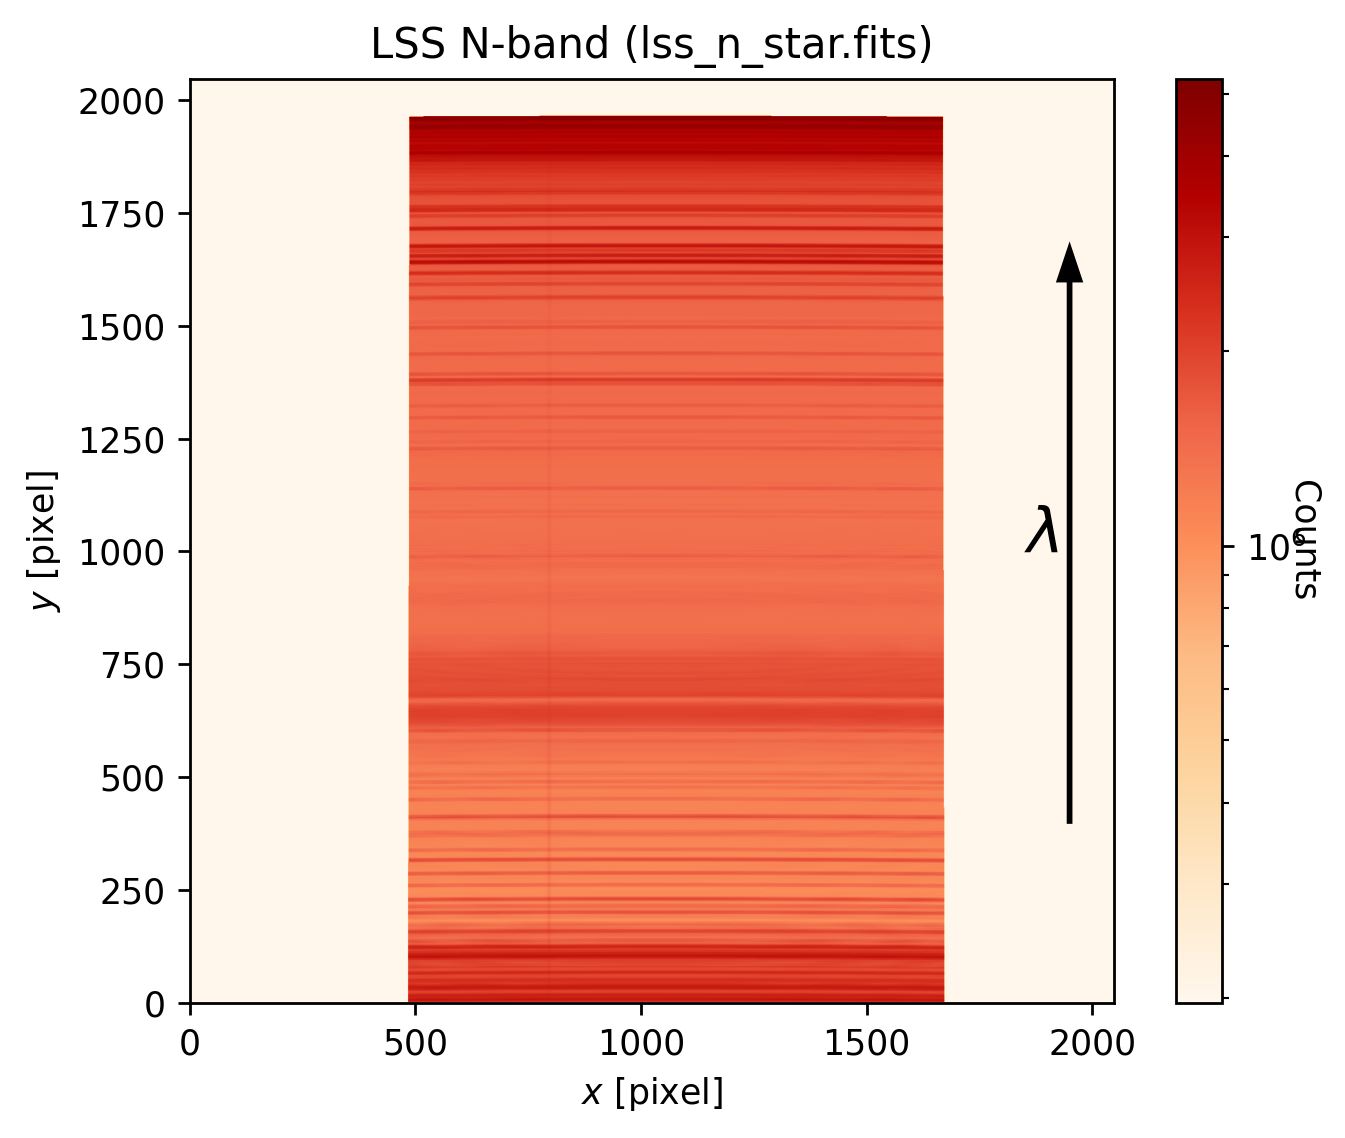
\includegraphics[height=4cm,keepaspectratio]{figures/LSS_CrtAlg_files/lss_n_star.fits}.png}
  \caption{Star spectrum ("science" target) frames for \lss~$L$-, $M$-, and $N$-bands.} 
  \label{fig:star}
\end{figure}

%-----------
\paragraph{Installing and running \pyred}\label{sec:pryred_install}

For the purpose of this report, we set up a git repository of a version of \pyred~adapted to work on simulated \met~data. This package can be downloaded from \url{https://github.com/nadsabha/PyReduce_ELT} or installed via Python~3 pip command: \\
\texttt{pip install git+https://github.com/nadsabha/PyReduce\_ELT} \\
The package includes a README file with instructions pertaining to running \pyred~on \elt~data and links to the needed input data (\texttt{README.md})).
% To display the feasibility of adopting \pyred~algorithms The package is so far adapted to work on one detector in the IJ-band short slit. Adaptations  which is 


%-----------
\paragraph{Order detection}\label{sec:critalg_orderdet}
%\todo[inline]{DONE-NS-210730: include report}

\begin{figure}[!ht]
  \centering
  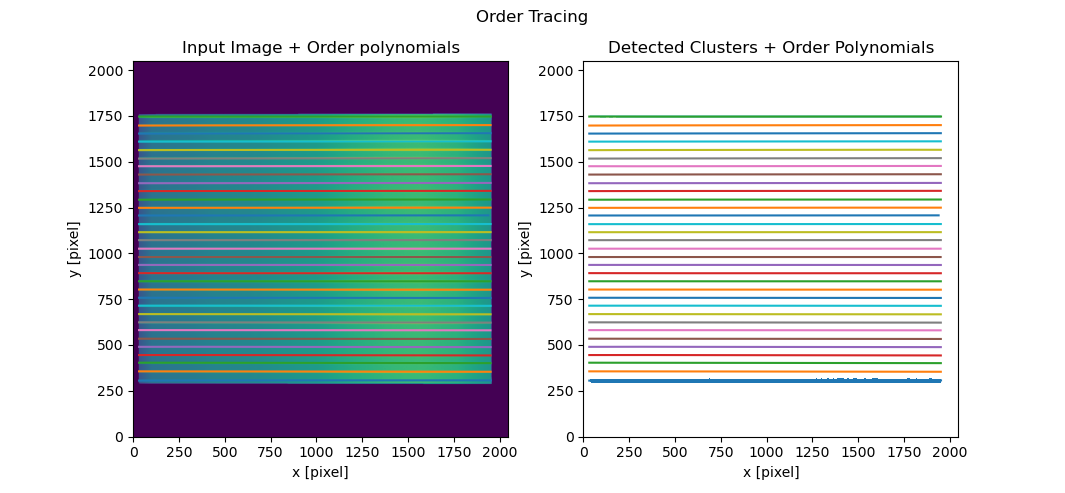
\includegraphics[width=\textwidth]{figures/LSS_CrtAlg_files/Figure_4.png}
  \caption{\textbf{\pyred~output}: Slit traces. Left panel: The fitted order polynomials overlaid on the image of the spectroscopic flat field with the pinholes. Right: The fitted order polynomials overlaid on the detected clusters for the order traces. For \met data, only the central polynomial trace for each trace is returned and used in the subsequent steps. Shown here for the case of \lss~$M$-band. }
  \label{fig:fig3}
\end{figure}

The details of how \pyred~handles the detection of the spectroscopic orders is described in Sect.~\ref{ssec:orderhandling} and \cite{pis02, pis21}. 
\pyred~rotates the images by 90 degrees counter clockwise to align the wavelength dispersion direction along the x-axis and performs the order detection on the pinhole frame with the flat field lamp.  Clusters of neighboring pixels belonging to an order trace are identified  and merged together according to predefined criteria. In the case of \met, a total of thirty three polynomials are fitted as order traces for each slit trace on the detector. These correspond to the pinhole positions of the flat field frame, see Fig.~\ref{fig:fig3}. To correctly extract the trace, the main routine \texttt{reduce.py} is modified to return only the central polynomial fit of each trace on the detector, i.e. fit number 17 (or 16 as per Python convention counted from bottom to up). This allowed a correct extraction of the traces in preparation for the curvature determination step. The order trace fits are stored in the \pyred~output file \texttt{metis\_lss\_m.ord\_default.npz} under \texttt{orders} and \texttt{column\_range} recarrays.
%-----------
\paragraph{Slit curvature}\label{sec:critalg_orderrect}
%\todo[inline]{DONE-NS-210730: include report}

\begin{figure}
\centering
  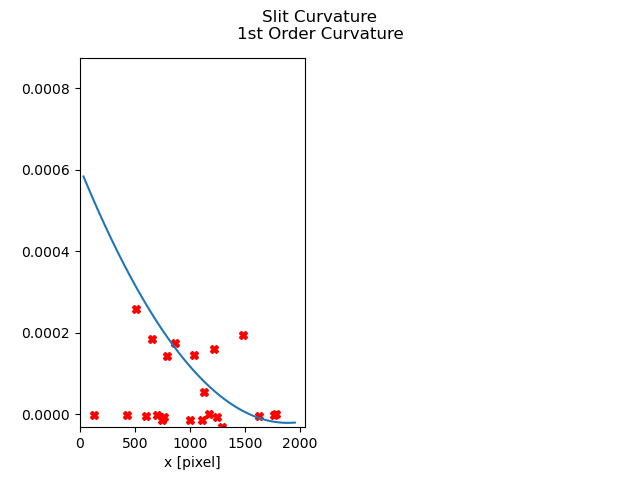
\includegraphics[width=\linewidth]{figures/LSS_CrtAlg_files/Figure_8.png}
  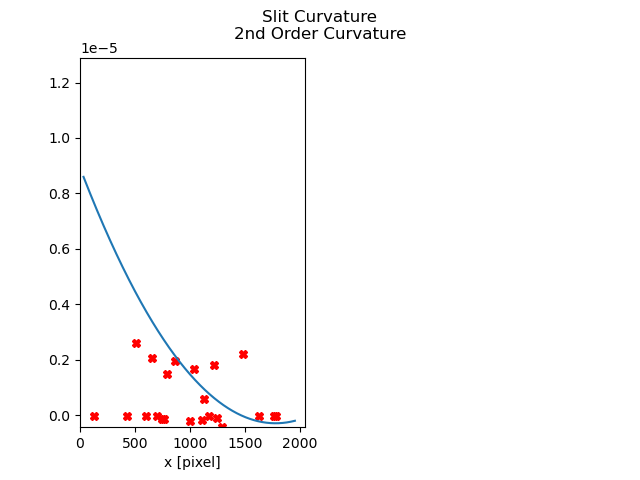
\includegraphics[width=\linewidth]{figures/LSS_CrtAlg_files/Figure_9.png}
  \caption{\textbf{\pyred~output}: Slit curvature tilt (1st order curvature) and shear (2nd order curvature) determination. Shown here for the case of \lss~$M$-band. } 
  \label{fig:fig6n7}
\end{figure}

\pyred~determines the slit curvature by identifying wavelength calibration spectral lines in the extracted order trace and fits the tilt and shear of each order along the image (1st order curvature and 2nd order curvature, respectively). More details on how the package handles slit curvature is discussed in Sect.~\ref{ssec:orderhandling} and \cite{pis21}. 

Figure~\ref{fig:fig6n7} shows the result of the polynomial fitting of the tilt and shear for the extracted slit trace of the \lss~$M$-band file \texttt{lss\_m\_sky.fits}. Figure~\ref{fig:fig8} shows the spectral lines used for the curvature determination  overlaid by the extracted tilt and shear marked in red lines. The x-axis corresponds to the y-axis on the original fits images (Fig~\ref{fig:sky}), while the y-axis of Fig.~\ref{fig:fig8} refers to the order trace number on the detector as \pyred~extracted it. Order~0 is the slit trace of the long slit. The order curvature polynomial fits are stored in the \pyred~output file \texttt{metis\_lss\_m.shear.npz} under \texttt{tilt} and \texttt{shear} recarrays.
\begin{figure}[!ht]
  \centering
  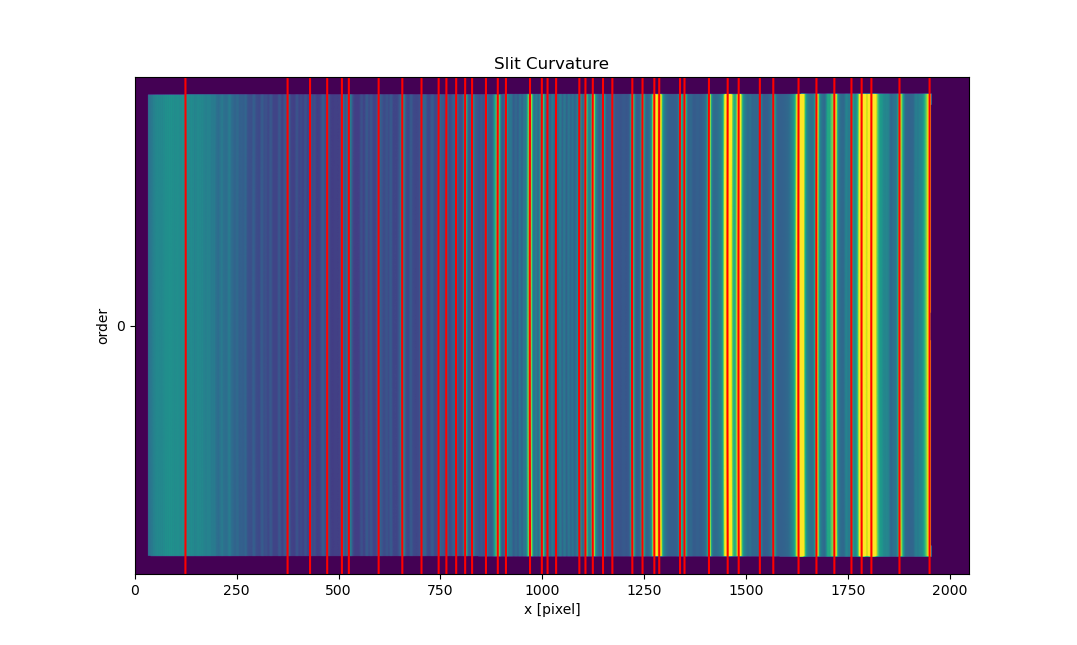
\includegraphics[width=\textwidth]{figures/LSS_CrtAlg_files/Figure_10.png}
  \caption{\textbf{\pyred~output}: Slit curvature determination. The spectral lines used for the curvature determination are overlaid by the extracted tilt and shear fits marked in red lines. Shown here for the case of \lss~$M$-band.}
  \label{fig:fig8}
\end{figure}

%-----------
\paragraph{Wavelength calibration}\label{sec:critalg_wavecal}
%\todo[inline]{DONE-NS-210730: include report}

The algorithm for the wavelength calibration strategy is described in Sect.~\ref{ssec:wavecal} and in \cite{pis02, pis21}. Here we describe and assess the performance of \pyred. 




\begin{figure}[!ht]
  \centering
  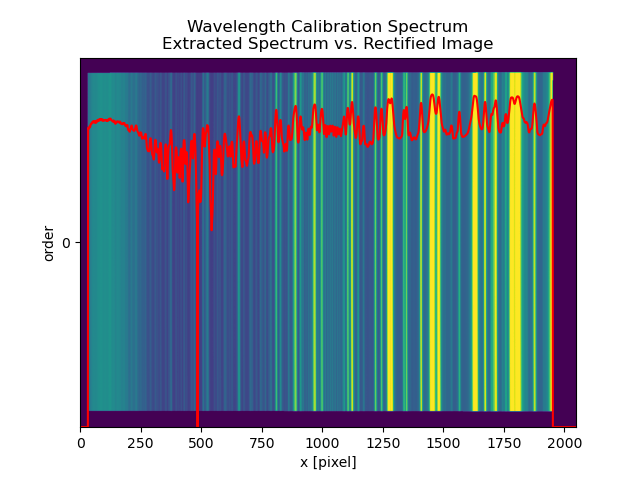
\includegraphics[width=\textwidth]{figures/LSS_CrtAlg_files/Figure_12.png}
  \caption{\textbf{\pyred~output}: Wavelength calibration extracted spectrum. Shown here for the case of \lss~$M$-band.}
  \label{fig:fig9}
\end{figure}

After the order tracing, extraction and curvature (tilt and shear) determination, \pyred~extracts can proceed with extracting a wavelength calibration spectrum for each order (here only one since we have an \lss~mode) from the wavelength calibration frame (\texttt{lss\_m\_sky.fits}, Fig.~\ref{fig:fig9}). The order spectrum is then compared to the wavelength calibration guess file \texttt{metis\_lss\_m\_2D.npz} of the \lss~$M$-band.  The \texttt{npz} file includes a numpy recarray called \texttt{cs\_lines} which lists mainly the wavelengths of the calibration reference lines, the x-pixel positions for start, center, and the end of each of the line traces on the detector, and the corresponding order as per \pyred~detection convention (here is zero in the case of \met~\lss). The list of reference lines and their positions on the detector was obtained by cross-matching their wavelengths  with the spectral layout of \met~\lss~for each band as obtained from the \met~IRDB\footnote{Instrument Reference Database, \url{https://github.com/AstarVienna/irdb/tree/dev_master/METIS}} and implemented in \scope~(e.g. \texttt{TRACE\_LSS\_M.fits}, see also Figure~\ref{fig:lmn_layout}). \pyred~then performs a cross-correlation to determine any offset between the reference (green lines) and the observation (red lines) as shown in \pyred~intermediate output file in Fig.~\ref{fig:fig10}.
\begin{figure}[!ht]
  \centering
  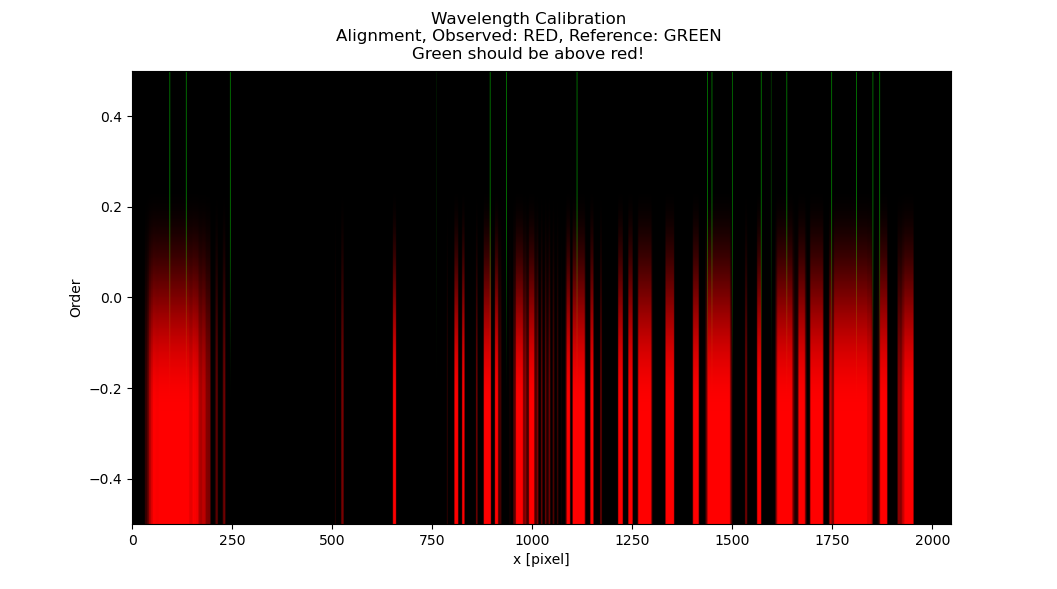
\includegraphics[width=\textwidth]{figures/LSS_CrtAlg_files/Figure_13.png}
  \caption{\textbf{\pyred~output}: Lines used for the wavelength calibration. The reference lines (green) and the observed lines (red) are aligned to each other for each order, where the green reference lines are shown to the top of the red observed line.  Shown here for the case of \lss~$M$-band.}
  \label{fig:fig10}
\end{figure}

Wavelength calibration residuals are then calculated for matching lines and a wavelength solution  is found. The wavelength solution for \met~\lss~is found by fitting a 2D polynomial, with degrees of 4 and 4 in the dispersion and the spatial direction, respectively. Figure~\ref{fig:fig12} bottom panel shows the 2D wavelength solution of the extracted slit trace where it can be seen that the wavelength range and increment of the trace match the spectral layout on detector one as seen in Fig.~\ref{fig:lmn_layout}.  The wavelength calibration spectrum is shown in the top panel of Fig.~\ref{fig:fig12}. The wavelength calibration spectrum is stored in the \pyred~output file \texttt{metis\_lss\_m.thar\_master.fits} and the corresponding wavelength solution in \texttt{metis\_lss\_m.thar.npz} recarrays \texttt{wave} and \texttt{coef}, while a modified list of the wavelength calibration lines is returned  in \texttt{linelist} indicating which line was used in the fitting procedure. 

\begin{figure}[!ht]
  \centering
  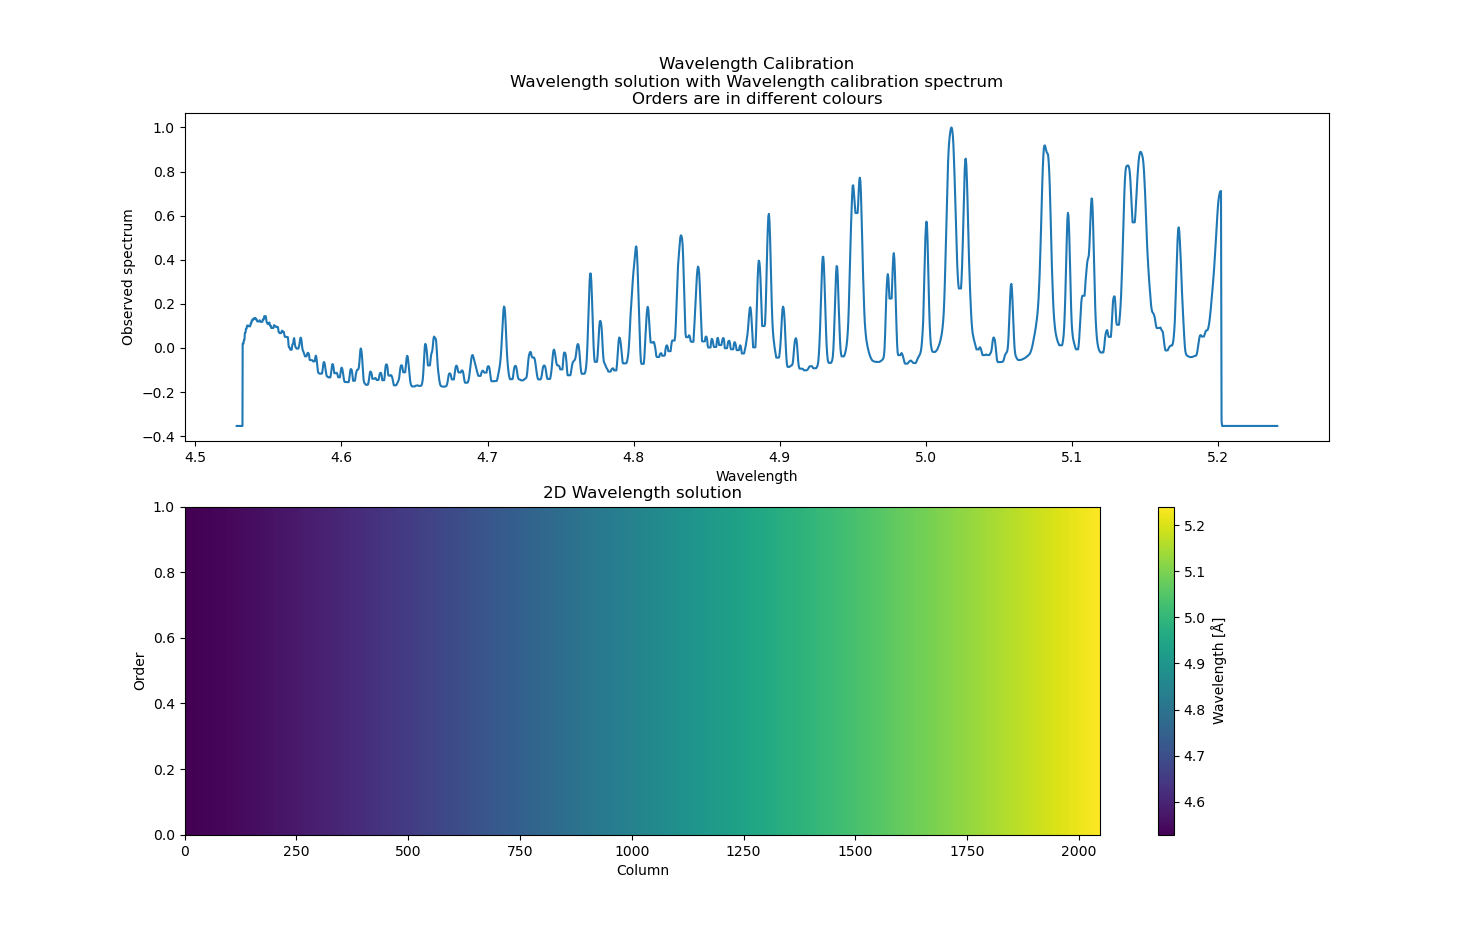
\includegraphics[width=\textwidth]{figures/LSS_CrtAlg_files/Figure_15.png}
  \caption{\textbf{\pyred~output}: Top: Wavelength calibration spectrum for  \lss~$M$-band. Bottom: 2D wavelength solution of \pyred~order~0 (\lss slit trace). The x-axis (Column) refers to the y pixel of the detector image in Fig.~\ref{fig:lmn_layout}. }
  \label{fig:fig12}
\end{figure}




To assess the accuracy of the wavelength solution, the extracted wavelength calibration spectrum is compared to the input sky spectrum \texttt{SKYCALC\_LSS\_override.fits} from \met~IRDB (see Figure~\ref{fig:sky_spec}). The sky spectrum is based on \textsc{Skycalc}, which is in turn based on \textsc{HITRAN}\footnote{\url{www.hitran.org}}. Figure~\ref{fig:r_m} top panel show the spectrum extracted by \pyred. The vertical dashed lines indicate the reference wavelength of each detected calibration sky line. The bottom panel shows the residuals between the reference wavelength and fitted wavelength (line center) of each detected calibration line divided by its $FWHM$. As can be seen, the calculated residuals are within $\pm 0.1 \times~FWHM$ for most lines.

\begin{figure}[!h]
  \centering
  \includegraphics[width=\textwidth]{figures/LSS_CrtAlg_files/{SKYCALC_LSS_override.fits}.png}
  \caption{\textbf{Input sky spectrum over the wavelength range covered by \met~\lss modes}: The sky spectrum is taken from \met~IRDB file \texttt{SKYCALC\_LSS\_override.fits}. }
  \label{fig:sky_spec}
\end{figure}

% \subparagraph{Wavelength calibration accuracy}\label{sec:critalg_wavecal_acc}
% \begin{figure}[!ht]
%   \centering
%   \includegraphics[width=0.8\textwidth]{figures/LSS_CrtAlg_files/Residuals_72.png}
%   \caption{Residuals of the wavelength calibration for \lss~$M$-band. The top panel displays the extracted wavelength calibration spectrum. The bottom panel shows the residuals of the wavelength calibration divided by the $FWHM$ of each respective line. The vertical dotted lines are the reference wavelengths of the input sky emission lines. }
%   \label{fig:r_m}
% \end{figure}

% \begin{figure}[!ht]
%   \centering
%   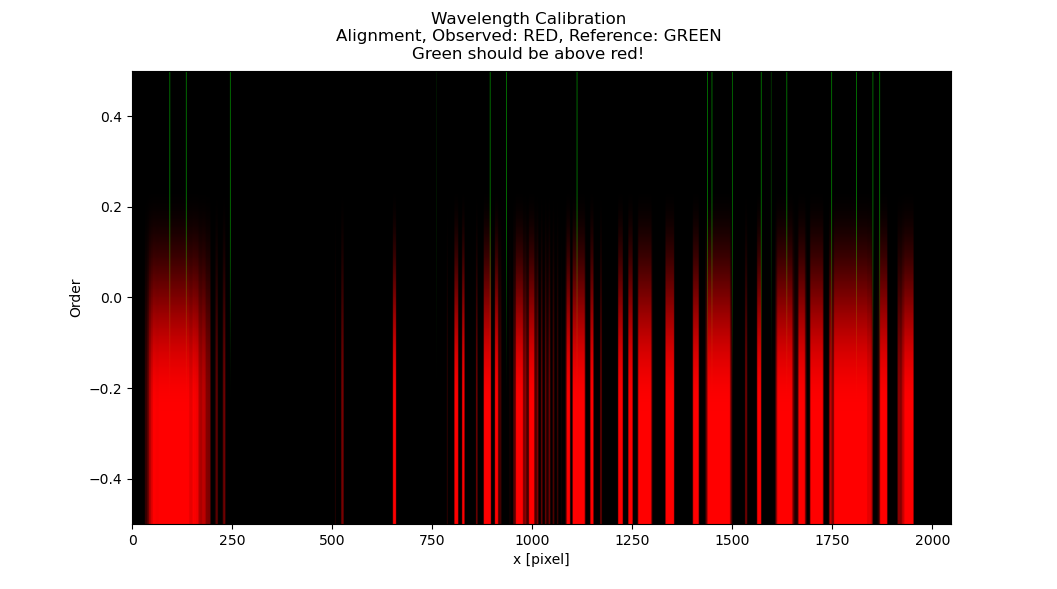
\includegraphics[width=\textwidth]{figures/LSS_CrtAlg_files/Figure_13.png}
%   \caption{\textbf{\pyred~output}: Extracted spectrum from a simulated science frame overlaid on the rectified order images. }
%   \label{fig:fig13}
% \end{figure}

% Figure~\ref{fig:fig13} shows the extracted and rectified spectrum from the frame \texttt{IJ\_freqcomb\_newheaders.fits} (Fig.~\ref{fig:star}) where an optimal extraction is performed using the \pyred~step \texttt{"science"}. 

\paragraph{Summary}
We showed  that the \pyred~package (currently part of CRIRES+ pipeline) can be adapted to work on simulated \met~\lss~data in all bands by creating the needed \pyred~files and tweaking the parameters used for each of the reduction steps (see linked package). All three steps of order detection, curvature determination, and wavelength calibration are successfully implemented. Further tweaking of certain parameters may be needed to improve the individual steps.


% The current setup of \pyred~assumes that each detector is to be treated individually, therefore we focused on adapting  it to the first detector of the IJ-band short slit. For a full implementation, we will create wavelength calibration guess files  for the remaining detectors, bands, and slits, to be treated in similar fashion to what we just showed. Alternatively for future prospects, one could consider combining all nine detectors into one large image by updating the instrument class and alternating one of the core routines of \pyred~that first reads the data and prepares it for the analysis (private communication with Ansgar Wehrhahn). 



% \TODO{Pyreduce, will be described by Nadeen.  IMG modes are not critical, see recipes.}

% \TODO{The old PDR text commented out. Todo can be removed}

%The MIR range is dominated by thermal and line emission in the Earth's atmosphere. These emission lines can be used to determine both, the curvature / tilt-distortion of the LSS spectrograph and subsequently the wavelength calibration in the following way: %(cf.\ Fig.\,\ref{fig:lm_lss_dist_wave}):

%\begin{itemize}
%  \item In a first step, atmospheric emission line peaks are detected in
%    detector rows in dispersion direction (green and yellow dots in in
%    Fig.\,\ref{fig:lm_lss_dist_wave}) (the same procedure might be
%    applied to absorption features).
%  \item Assuming that these peaks are located in the very neighborhood
%    in dispersion direction, it is possible to cross identifying them on
%    each of the pixel rows (yellow dots in
%    Fig.\,\ref{fig:lm_lss_dist_wave}).
%  \item The distortion along a line is then determined by fitting a
%    polynomial (e.g.\ Chebyshev polynomial) along these associated
%    points (purple line).  This polynomial solution might rely on first
%    guesses for the distortions introduced by the fixed ADCs and is used
%    to determine the rectification. The WCU lamp spectrum might provide
%    a 0\textsuperscript{th}-order guess, which is refined with a table,
%    which includes information on the distortion introduced by the
%    grisms (\STATCALIB{GRISM_TAB}).
%  \item Since we know the wavelength range (from the optical system), a
%    cross correlation of the lines with respect to the molecular
%    emission lines from line databases
%    (e.g.\ HITRAN\footnote{\url{https://hitran.org/}},
%    \STATCALIB{ATM_LINE_CAT}) is possible.
%\end{itemize}

%Special emphasis has to be drawn that the rows to detect the atmospheric emission lines are not to cover the science objects, since intrinsic target emission lines might disturb the cross correlation.

%\begin{figure}[ht]
%  \centering
%  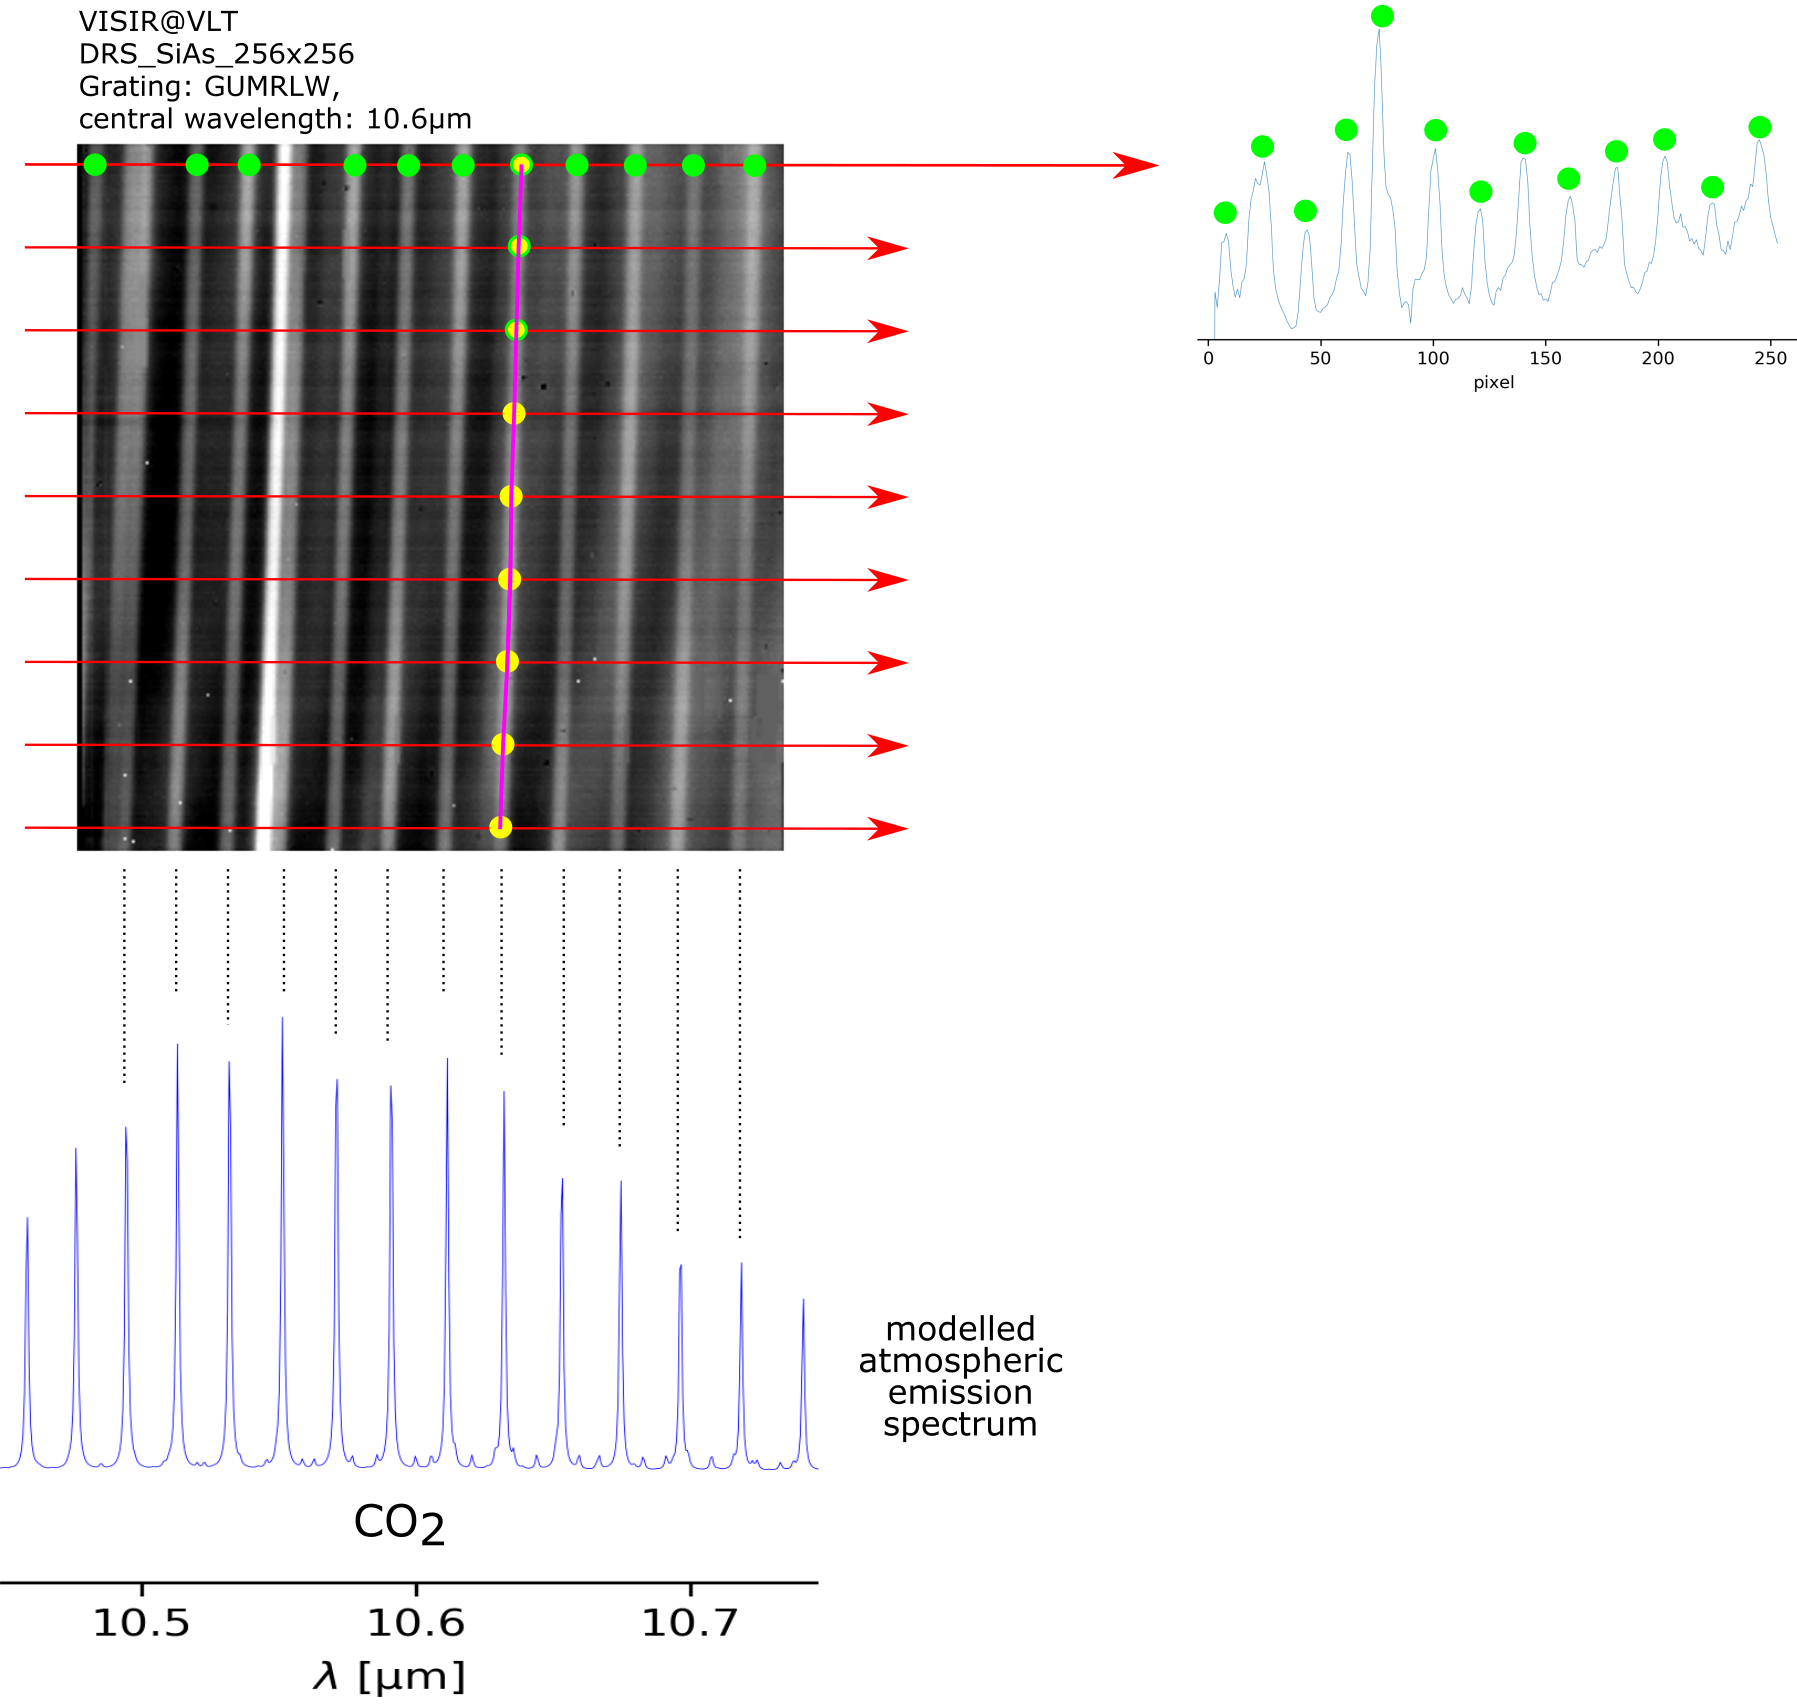
\includegraphics[width=0.6\textheight]{wavecal_distortion.png}
%  \caption[Algorithm for wavelength calibration and distortion determination]{%
%    Sketch of the intended algorithm for the wavelength calibration
%    and distortion determination (raw VISIR@VLT frame). Emission lines
%    arising from our Earth's atmosphere can be used to determine the
%    wavelength calibration and the distortions (see text for more
%    details).\TODO{REMOVE THIS OBSOLETE FIGURE}}
%  \label{fig:lm_lss_dist_wave}
%\end{figure}

\subsubsection{IFU distortion correction}\label{ssec:criticalwavelengthanddistortionifu}
The following is a summary of the steps that were taken to apply the
CRIRES+ data reduction to simulation the METIS LMS IFU.
\begin{itemize}
    \item ScopeSim runs
    \item Insert data into CRIRES frames
    \item Order tracing
    \item Tilt determination
    \item Extracting 1D spectra
    \item Assigning Wavelength and spatial scale to pixels in 2D spectra
\end{itemize}

\paragraph{ScopeSim}
As of April 2022, when these simulations were carried out, the
release-version of the simulator did not support the IFU mode of METIS.
Therefore a development version of the LMS-branch was istalled, after
instructions from the team. The mode was set such that the The scipt
that creates the frame with the sky spectrum is called
\texttt{lms\_sky.py} and does very little besides calling the simulator
with default arguments, and instructing it to set the central wavelength
of the spectrograph to arbitrary $3.55$ micron. In addition, it retrieves
the wavelength scale from one of the slices, in order to later ingest it
into the CRIRES-pipeline.

\paragraph{CRIRES DRS}
The upgraded CRIRES is a cross-dispersed echelle slit-spectrograph for
the near-infrared bands YJHKLM. It uses three of the same HAWAII2RG
detectors that METIS will use four of. The fact that CRIRES images
several spectral orders while METIS does slices of spatial regions, is
no hindrance to applying the same methods for finding the location and
shape of each order/slice in the detector grid, and to determine the
orientation of the ``slit''.

The CRIRES DRS is a standard ESO-pipeline that was developped from
scratch for the upgraded instrument and is in operation since late 2021.
It can be installed from the usual sources for ESO pipelines on their
website, no particular version is needed for this exercise since the
basic algorithms have not changed.

ScopeSim produces frames for all four of the LMS detectors. Simply
ignoring the fourth, the pixel values were copied into a raw frame
CRIRES, thus preserving its headers and replacing the data.

\paragraph{Order tracing}

By ``trace'' we mean the polynomial in detector coordinates (x,y) that
describes the mid-line of the spectral order. This is done by smoothing
and thresholding the sky frame (which has enough continuum) in order to
distinguish in-order from inter-order pixels. Continuous clusters of
in-order pixels are then fitted with a second-degree polynomial. The
command executed was

\begin{verbatim}
# esorex cr2res_util_trace trace_sky.sof
\end{verbatim}

where \texttt{trace\_sky.sof} contains only one line, pretending the
sky frame is a FLAT (which is what is usually used for tracing)

\begin{verbatim}
CIRES_sky.fits FLAT
\end{verbatim}

The output file is \texttt{CIRES\_sky\_tw.fits} which is a table that
now has the traces for each slice. In addition to the mid-line, it also
has the polynomials for the upper and lower edges of each slice.

\paragraph{Slit tilt}

Next up is measuring the orientation of the ``slit'' in each slice,
i.e.~the tilt of spectral lines w.r.t. the detector columns. Using the
trace from the previous step, each slice gets rectified by shifting
columns by integer values according to the trace.

Then a peak-finder is run on each row to find spectral lines, which are
then fitted with Gaussians to determine their line centers. Comparing
how the line-centers change with detector rows, allows us to fit the
slit tilt as a polynomyal P(y). In order to reject outliers and ensure a
smooth change in the tilt, the \emph{coefficients} of the tilt
polynomials are then each fit as P(x).

These coefficients are saved in an updated FITS-table, called
\texttt{CIRES\_sky\_tw\_tw.fits}. Using the included script that
evaluates the polynomials and plots them on top of the sky frame, we can
have a look at the result.

    \begin{tcolorbox}[breakable, size=fbox, boxrule=1pt, pad at break*=1mm,colback=cellbackground, colframe=cellborder]
\prompt{In}{incolor}{25}{\boxspacing}
\begin{Verbatim}[commandchars=\\\{\}]
\PY{o}{\PYZpc{}}\PY{k}{run} show\PYZus{}trace\PYZus{}curv.py CIRES\PYZus{}sky\PYZus{}tw\PYZus{}tw.fits CIRES\PYZus{}sky.fits
\PY{c+c1}{\PYZsh{} (This plots only the top row of two detectors)}
\end{Verbatim}
\end{tcolorbox}

\begin{center}
\adjustimage{max size={0.9\linewidth}{0.9\paperheight}}{LMS distortion_files/LMS distortion_7_0.png}
\end{center}
{ \hspace*{\fill} \\}

\begin{tcolorbox}[breakable, size=fbox, boxrule=1pt, pad at break*=1mm,colback=cellbackground, colframe=cellborder]
\prompt{In}{incolor}{26}{\boxspacing}
\begin{Verbatim}[commandchars=\\\{\}]
\PY{c+c1}{\PYZsh{} Zooming in allows to perceive the tilt in the regularly plotted vertical lines that align with the data.}
\PY{k+kn}{from} \PY{n+nn}{IPython}\PY{n+nn}{.}\PY{n+nn}{display} \PY{k}{import} \PY{n}{Image}\PY{p}{,} \PY{n}{display}
\PY{n}{display}\PY{p}{(}\PY{n}{Image}\PY{p}{(}\PY{n}{filename}\PY{o}{=}\PY{l+s+s1}{\PYZsq{}}\PY{l+s+s1}{lms\PYZus{}sky\PYZus{}tracetilt\PYZus{}zoom.png}\PY{l+s+s1}{\PYZsq{}}\PY{p}{)}\PY{p}{)}
\end{Verbatim}
\end{tcolorbox}

\begin{center}
\adjustimage{max size={0.9\linewidth}{0.9\paperheight}}{LMS distortion_files/LMS distortion_8_0.png}
\end{center}
{ \hspace*{\fill} \\}

\begin{tcolorbox}[breakable, size=fbox, boxrule=1pt, pad at break*=1mm,colback=cellbackground, colframe=cellborder]
\prompt{In}{incolor}{27}{\boxspacing}
\begin{Verbatim}[commandchars=\\\{\}]
\PY{n}{tilts} \PY{o}{=} \PY{n}{fo}\PY{p}{(}\PY{l+s+s1}{\PYZsq{}}\PY{l+s+s1}{CIRES\PYZus{}sky\PYZus{}tw\PYZus{}tw.fits}\PY{l+s+s1}{\PYZsq{}}\PY{p}{)}\PY{p}{[}\PY{l+m+mi}{1}\PY{p}{]}\PY{o}{.}\PY{n}{data}\PY{p}{[}\PY{l+s+s1}{\PYZsq{}}\PY{l+s+s1}{SlitPolyB}\PY{l+s+s1}{\PYZsq{}}\PY{p}{]}
\PY{n}{tilts}
\end{Verbatim}
\end{tcolorbox}

\begin{tcolorbox}[breakable, size=fbox, boxrule=.5pt, pad at break*=1mm, opacityfill=0]
\prompt{Out}{outcolor}{27}{\boxspacing}
\begin{Verbatim}[commandchars=\\\{\}]
array([[-1.45030918e-02,  4.97644175e-06, -8.81093015e-10],
       [-1.71465266e-02,  1.19526702e-05, -4.11230539e-09],
       [-1.60470680e-02,  9.62834066e-06, -2.46179182e-09],
       [-1.56843290e-02,  1.04739179e-05, -3.39557250e-09],
       [-9.89049691e-03, -7.80064422e-07,  1.55907143e-09],
       [-1.37041189e-02,  7.36109573e-06, -1.76092183e-09],
       [-1.21335419e-02,  3.73431498e-06,  3.62338925e-10],
       [-9.88651568e-03,  1.90595104e-06,  9.70922842e-10],
       [-1.25626738e-02,  9.42000943e-06, -3.06478176e-09],
       [-1.23701034e-02,  4.81279417e-06,  6.75878571e-10],
       [-1.30267035e-02,  9.46268944e-06, -2.61068479e-09],
       [-9.47728454e-03,  3.20871517e-06,  1.27630431e-09],
       [-1.29999200e-02,  1.02179873e-05, -1.89150864e-09],
       [-1.04358752e-02,  2.52729614e-06,  1.30881039e-09]])
\end{Verbatim}
\end{tcolorbox}

When we evaluate one of the polynomials at the detector edges and
center, we find that the slit angle varies between 0.5 and 0.9 degrees.

\begin{tcolorbox}[breakable, size=fbox, boxrule=1pt, pad at break*=1mm,colback=cellbackground, colframe=cellborder]
\prompt{In}{incolor}{28}{\boxspacing}
\begin{Verbatim}[commandchars=\\\{\}]
\PY{n}{dx}\PY{o}{=}\PY{n}{np}\PY{o}{.}\PY{n}{polyval}\PY{p}{(}\PY{n}{tilts}\PY{p}{[}\PY{l+m+mi}{3}\PY{p}{]}\PY{p}{[}\PY{p}{:}\PY{p}{:}\PY{o}{\PYZhy{}}\PY{l+m+mi}{1}\PY{p}{]}\PY{p}{,}\PY{p}{[}\PY{l+m+mi}{1}\PY{p}{,}\PY{l+m+mi}{1024}\PY{p}{,}\PY{l+m+mi}{2048}\PY{p}{]}\PY{p}{)} \PY{c+c1}{\PYZsh{} reverse order of coeffs in python}
\PY{n}{dx}
\end{Verbatim}
\end{tcolorbox}

\begin{tcolorbox}[breakable, size=fbox, boxrule=.5pt, pad at break*=1mm, opacityfill=0]
\prompt{Out}{outcolor}{28}{\boxspacing}
\begin{Verbatim}[commandchars=\\\{\}]
array([-0.01567386, -0.00851955, -0.00847581])
\end{Verbatim}
\end{tcolorbox}

\begin{tcolorbox}[breakable, size=fbox, boxrule=1pt, pad at break*=1mm,colback=cellbackground, colframe=cellborder]
\prompt{In}{incolor}{29}{\boxspacing}
\begin{Verbatim}[commandchars=\\\{\}]
\PY{n}{np}\PY{o}{.}\PY{n}{degrees}\PY{p}{(}\PY{n}{np}\PY{o}{.}\PY{n}{arctan}\PY{p}{(}\PY{n}{dx}\PY{p}{)}\PY{p}{)} \PY{c+c1}{\PYZsh{} Tilt angles}
\end{Verbatim}
\end{tcolorbox}

\begin{tcolorbox}[breakable, size=fbox, boxrule=.5pt, pad at break*=1mm, opacityfill=0]
\prompt{Out}{outcolor}{29}{\boxspacing}
\begin{Verbatim}[commandchars=\\\{\}]
array([-0.89797241, -0.48812261, -0.48561642])
\end{Verbatim}
\end{tcolorbox}

\begin{tcolorbox}[breakable, size=fbox, boxrule=1pt, pad at break*=1mm,colback=cellbackground, colframe=cellborder]
\prompt{In}{incolor}{30}{\boxspacing}
\begin{Verbatim}[commandchars=\\\{\}]
\PY{n}{dx}\PY{o}{*}\PY{l+m+mi}{80} \PY{c+c1}{\PYZsh{} pixel difference between top and bottom of a slice, \PYZti{}80pix high}
\end{Verbatim}
\end{tcolorbox}

\begin{tcolorbox}[breakable, size=fbox, boxrule=.5pt, pad at break*=1mm, opacityfill=0]
\prompt{Out}{outcolor}{30}{\boxspacing}
\begin{Verbatim}[commandchars=\\\{\}]
array([-1.25390868, -0.68156423, -0.67806467])
\end{Verbatim}
\end{tcolorbox}

\paragraph{Extracting into 1D spectra}
Before we use the ``TW''-table from above to extract 1D-spectra, we need
to fix the wavelength scale that is also part of the table (TW stands
for TraceWave-table in CRIRES-lingo), because otherwise the spectra
would have a totally wrong wavelengh scale. For simplicity, the
numbering of the METIS slices was not matched with the CRIRES numbering
of orders, instead we set the wavelength of one slice (saved into
\texttt{lam\_1.npy} by the script above) for all spectra of the same
detector.

    \begin{tcolorbox}[breakable, size=fbox, boxrule=1pt, pad at break*=1mm,colback=cellbackground, colframe=cellborder]
\prompt{In}{incolor}{31}{\boxspacing}
\begin{Verbatim}[commandchars=\\\{\}]
\PY{n}{tw}\PY{o}{=}\PY{n}{fo}\PY{p}{(}\PY{l+s+s1}{\PYZsq{}}\PY{l+s+s1}{CIRES\PYZus{}sky\PYZus{}tw\PYZus{}tw.fits}\PY{l+s+s1}{\PYZsq{}}\PY{p}{)}
\PY{k}{for} \PY{n}{detec} \PY{o+ow}{in} \PY{p}{[}\PY{l+m+mi}{1}\PY{p}{,}\PY{l+m+mi}{2}\PY{p}{]}\PY{p}{:}
    \PY{n}{lam}\PY{o}{=}\PY{n}{np}\PY{o}{.}\PY{n}{load}\PY{p}{(}\PY{l+s+s1}{\PYZsq{}}\PY{l+s+s1}{lam\PYZus{}}\PY{l+s+si}{\PYZpc{}d}\PY{l+s+s1}{.npy}\PY{l+s+s1}{\PYZsq{}}\PY{o}{\PYZpc{}}\PY{k}{detec})
    \PY{n}{x}\PY{o}{=}\PY{n}{np}\PY{o}{.}\PY{n}{arange}\PY{p}{(}\PY{n+nb}{len}\PY{p}{(}\PY{n}{lam}\PY{p}{)}\PY{p}{)}\PY{o}{+}\PY{l+m+mi}{1} 
    \PY{n}{p}\PY{o}{=}\PY{n}{np}\PY{o}{.}\PY{n}{polyfit}\PY{p}{(}\PY{n}{x}\PY{p}{,}\PY{n}{lam}\PY{p}{,}\PY{l+m+mi}{2}\PY{p}{)}\PY{p}{[}\PY{p}{:}\PY{p}{:}\PY{o}{\PYZhy{}}\PY{l+m+mi}{1}\PY{p}{]}
    \PY{n+nb}{print}\PY{p}{(}\PY{n}{p}\PY{p}{)}
    \PY{k}{for} \PY{n}{row} \PY{o+ow}{in} \PY{n}{tw}\PY{p}{[}\PY{l+s+s1}{\PYZsq{}}\PY{l+s+s1}{CHIP}\PY{l+s+si}{\PYZpc{}d}\PY{l+s+s1}{.INT1}\PY{l+s+s1}{\PYZsq{}}\PY{o}{\PYZpc{}}\PY{k}{detec}].data:
        \PY{n}{row}\PY{p}{[}\PY{l+s+s1}{\PYZsq{}}\PY{l+s+s1}{Wavelength}\PY{l+s+s1}{\PYZsq{}}\PY{p}{]}\PY{o}{=}\PY{n}{p}
\PY{n}{tw}\PY{o}{.}\PY{n}{writeto}\PY{p}{(}\PY{n}{tw}\PY{o}{.}\PY{n}{filename}\PY{p}{(}\PY{p}{)}\PY{p}{,}\PY{n}{overwrite}\PY{o}{=}\PY{k+kc}{True}\PY{p}{)}
\end{Verbatim}
\end{tcolorbox}

    \begin{Verbatim}[commandchars=\\\{\}]
[ 3.55110788e+00  1.28761289e-05 -5.17343629e-11]
[ 3.52304458e+00  1.29677244e-05 -2.01943107e-11]
    \end{Verbatim}

The following command runs the optimal extraction which collapses the
full height of each slice into a 1D-spectrum, taking the trace and slit
tilt into account and iterating to minimize the residual error. (We
arbitrarily select ``order \#3''; again this is CRIRES-numbering and has
no meaning for the purpose of this exercise.)

\begin{verbatim}
# esorex cr2res_util_extract --detector=1 --order=3 --trace=1 extract_sky.sof
\end{verbatim}

Now we can plot the spectrum from SkyCalc, that was used by ScopeSim,
against the our extracted spectrum. For size considerations, the input
sky spectrum is not included in this package and we display the pre-made
figure here.

    \begin{tcolorbox}[breakable, size=fbox, boxrule=1pt, pad at break*=1mm,colback=cellbackground, colframe=cellborder]
\prompt{In}{incolor}{32}{\boxspacing}
\begin{Verbatim}[commandchars=\\\{\}]
\PY{n}{display}\PY{p}{(}\PY{n}{Image}\PY{p}{(}\PY{n}{filename}\PY{o}{=}\PY{l+s+s1}{\PYZsq{}}\PY{l+s+s1}{lms\PYZus{}skyrecover.png}\PY{l+s+s1}{\PYZsq{}}\PY{p}{)}\PY{p}{)}
\end{Verbatim}
\end{tcolorbox}

\begin{center}
    \adjustimage{max size={0.9\linewidth}{0.9\paperheight}}{LMS distortion_files/LMS distortion_17_0.png}
\end{center}
{ \hspace*{\fill} \\}

In blue the input spectrum, in orange and green the spectra from the two
detectors that cover the slice. Vertical offset and scaling are
arbitrary. The slight offset in wavelength is due to the mismatch in
slice number between the assigned wavelength and the one that got
extracted. This nicely illustrates the task of the wavelength
calibration, namely to determine this shift by cross-correlation, but
this in not part of the current exercise.

\paragraph{2D spectra}
Collapsing slices (or parts of one) into 1D spectra is certainly useful,
not the least for calibrations. But METIS is all about spatial
resolution, of course, so this whole exercise would be incomplete
without assigning to each pixel a wavelength and a speatial coordinate
along the slice. Luckily, this is quite straight-forward from the
information in the TW-table. The polynomials for the slice edges and
mid-line, together with the known on-sky length of the slice, define the
position of each pixel on the sky. To arrive at the correct wavelenth,
one evaluates the slit-tilt polynomial at the current pixel's distance
from the mid-line, to get the displacement in dispersion direction. Then
this delta-x gets converted to delta-lambda using the wavelength
solution.

\begin{tcolorbox}[breakable, size=fbox, boxrule=1pt, pad at break*=1mm,colback=cellbackground, colframe=cellborder]
    \prompt{In}{incolor}{33}{\boxspacing}
\begin{Verbatim}[commandchars=\\\{\}]
\PY{c+c1}{\PYZsh{} plot missing, due to technical difficulties, this is a stand\PYZhy{}in from CRIRES\PYZhy{}data.}
\PY{n}{display}\PY{p}{(}\PY{n}{Image}\PY{p}{(}\PY{n}{filename}\PY{o}{=}\PY{l+s+s1}{\PYZsq{}}\PY{l+s+s1}{crires\PYZus{}2d\PYZus{}rect.png}\PY{l+s+s1}{\PYZsq{}}\PY{p}{)}\PY{p}{)}
\end{Verbatim}
\end{tcolorbox}

\begin{center}
    \adjustimage{max size={0.9\linewidth}{0.9\paperheight}}{LMS distortion_files/LMS distortion_20_0.png}
\end{center}
{ \hspace*{\fill} \\}

Any non-linear spatial distortion along the slice, as measured from the
full field-of-view of the LM-Imager, or by illuminating the IFU slices
with the grid of the pin-hole mask in the WCU, can be added to the
spatial scale as a last step.



\subsection{Telluric correction}\label{ssec:criticaltelluriccorrection}
Telluric correction, i.e. the removal of absorption features arising in the Earth's atmosphere,
is a critical issue as the imprint of molecular species present in our air may vary on different timescales
down to minutes, as the composition of the atmosphere may change over time.
In particular the \ac{MIR} range is affected (see App~\ref{app:atmo_trans}).

There are two well established ways to correct for these absorptions:
\begin{itemize}
    \item \textit{Classical approach}: A telluric standard star (\ac{TSS}) spectrum is taken ideally directly before/after the science observations at the same airmass. This \ac{TSS}-spectrum is processed in the same way as the science spectrum (except the absolute flux calibration) and finally its continuum is normalised to unity. In addition, a model of this specific \ac{TSS} spectrum is used to remove intrinsic spectral features. The remaining normalised spectrum (ideally) only contains the fingerprint of the Earth's atmospheric absorptions and can be used for the telluric correction. In case the model spectrum also contains absolute flux values, this star could also be appropriate for the absolute flux calibration.
    \item \textit{Modelling approach}: In the last years a new method has evolved which is based on radiative transfer modelling of the Earth's atmosphere (\cite{mf1, mf2, molecfit}\footnote{\url{https://www.eso.org/sci/software/pipelines/skytools/molecfit}}). A model of the Earth's atmosphere (probably refined with on-site measurements, e.g. with a radiometer measuring the \ac{PWV} profile along the line-of-sight) in combination with a radiative transfer model and a molecular line list containing lines of various species is used to determine the transmission of the Earth's atmosphere at the time of observations by fitting specific molecular absorption features in the science spectra. The best-fit transmission function is finally used for the telluric correction.
\end{itemize}
These two methods can also be combined in the way that the modelling approach is applied to a \ac{TSS} spectrum, and the resulting transmission function is then applied to the science spectrum. This combination is specifically useful if the science target continuum is too weak to use the absorptions for a fit.\\
For the \ac{METIS} pipelines we intend to incorporate both ways (including their combination). A detailed description is given in Section~\ref{ssec:tellcorr}. As both methods are well established, we deem a dedicated prototyping not necessary.

\subsection{Error propagation}\label{ssec:criticalerrorpropagation}
\label{Sec:critalg_errorprop}

All data products from the pipeline will be accompanied by an
estimate of the uncertainty in the derived values in the data products, in compliance with \REQ{METIS-6681}.

Error estimates are necessary for the scientific
exploitation of the data. They make it possible to assign
significances to detections and to estimate errors on photometric and
other measurements in the course of the scientific analysis of the
images. The uncertainties include noise contributions from photon
noise associated with the photon counting process over the integration
time of an exposure, dark current noise, detector read-out noise,
digitization noise, and possibly other sources.

The basic reduction procedures, such as dark subtraction and
flat-field correction, add the noise from calibration images to the
noise of the science exposures. These noise contributions need to be
tracked through the reduction process by applying standard error
propagation algorithms.

For this purpose, the DRS will make extensive use of \ac{HDRL} data structures.
These include built-in error propagation, for example HDRL-images have separate
layers for pixel values, their error and a mask. These are used automatically
when performing operations on images, such that the result has the propagated
error attached. In cases where this is not sufficient, errors will be calculated
manually.

Photon noise is the major noise component of mid-infrared data. The
number of electrons, $N_{e}$ libreated in a detector pixel over the
exposure time follows a Poisson distribution with variance $\sigma^{2}
= \langle N_{e}\rangle$, where $\langle N_{e}\rangle$ is the expected
number of electrons.

Pixel values $F$ in a raw image are given in ADU and are related to
the number of electrons via the gain factor $g$ (in
$\mathrm{e}^{-}/\mathrm{ADU}$):
\begin{equation}
  \label{eq:gain_def}
  F = g N_{e}.
\end{equation}
The expected noise in the image is thus
\begin{equation}
  \label{eq:noise_adu}
  \sigma_{F} = g\sqrt{\langle N_{e}\rangle} = \sqrt{g \langle F\rangle}.
\end{equation}

It is a mistake to estimate the expected count rate $\langle F\rangle$
by the actual count rate $F$ for each pixel. For a flux constant in
space and time this method would give a different estimate
$\sigma_{F}$ for each pixel in the same exposure, and also for the same pixel
in different exposures. This in turn leads to the undesirable result
that the weighted mean of several exposures $i = 1,\dots, N$ is biased
low as pixel values (drawn from a Poisson distribution) lower than the
expectation are systematically given larger weight than high pixel
values:
\begin{equation}
  \label{eq:weighted_mean}
  \overline{F} = \frac{\sum_{i=1}^{N}
    F_{i}/\sigma_{i}^{2}}{\sum_{i=1}^{N} 1/\sigma_{i}^{2}} =
  \frac{N}{\sum_{i=1}^{N}1/F_{i}} < \langle F\rangle
\end{equation}

Photon noise from thermal or sky background is therefore estimated
from a constant or low-order polynomial fit of the background estimate
in order to suppress random pixel fluctuations.

Pixel-wise modulation is introduced by the master flat field as this
quantifies the response of pixels to a constant background flux.

\subsection{N-band image restoration}
\label{ssec:criticalnbandimagerestoration}
\label{ssec:image_restoration}

% \TODO{
% Chop-nod inversion and stacking. Look at how VISIR does this.
% Need to look at sub-pixel chop shifts, and whether the images need to be resampled.
% Plate scale distortions are not really a issue, because we only care about compact objects.}

Images in the N band are taken in a sequence of chopped and nodded
exposures. The combination of these exposures results in an image with
one or more positive and negative images (``beams'') of the target
source, depending on the pattern of chops and nods. Image restoration
refers to an algorithm to process the chop-nod difference image into
an image where the various beams are combined into a single beam,
providing an increased signal-to-noise ratio.

The VISIR pipeline employs a shift-and-add algorithm with proper
inversion of the negative beams that works well for compact sources.
More elaborate algorithms have been
described that are also claimed to work for extended sources.

However, extended sources have been excluded from the scope of the pipeline.
No prototype is therefore provided.

% We will
% investigate these algorithms until FDR, taking into account the
% results of the investigations into background strategies that are
% on-going within the METIS consortium.

\subsection{IFU image and cube reconstruction}
\label{ssec:criticalifuimageandcubereconstruction}
\label{ssec:image_reconstruction}

Due to the width of the slices in the LM integral-field spectrograph
of 20.7\,mas, the PSF is undersampled in the across-slice direction.
In order to fully sample the PSF, the following observing sequence is envisaged:
\begin{itemize}
    \item Take three exposures, each offset perpendicular to the slice by a third of the slice width.
    % Maybe this could be more than a third, for instance 4/3 or 10/3, in order to help eliminate bad pixels:
    % The same model pixel would be always covered by three distinct hardware pixels
    \item Rotate the field by 90 degrees (with the derotator).
    \item Take three more exposures with the same across-slice dither pattern.
\end{itemize}

The pattern is visualised in Fig.~\ref{fig:ifu_pattern}. In principle,
this pattern yields a sampling of the field at a third of the slice
width (i.e.~7\,mas) in both spatial directions, which would be
sufficient for a full sampling of the PSF. How to implement this
reconstruction and to what extent the information can be recovered
from real data needs to be investigated.

\begin{figure}[hb]
  \centering
  \resizebox{0.8\textwidth}{!}{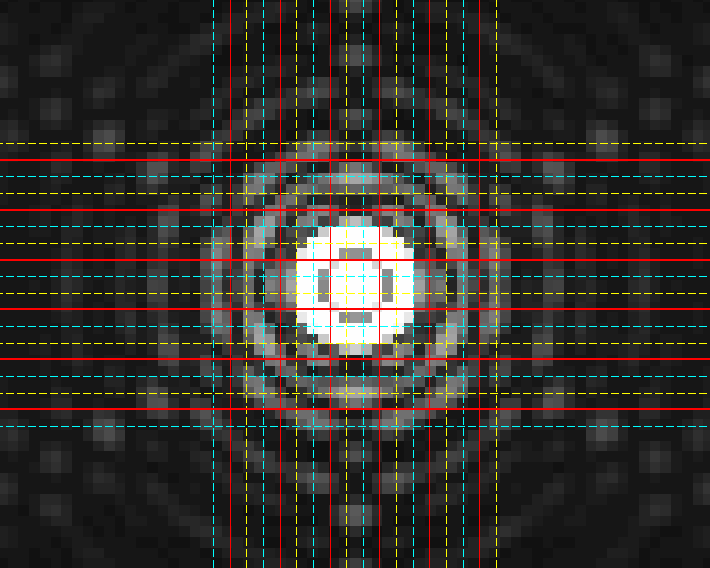
\includegraphics{PSF_IFU_slices}}
  \caption[IFU dithering and rotation pattern]{%
    IFU observation pattern overlaid on a METIS SCAO PSF (by Marcus
    Feldt, MPIA). Red horizontal lines mark the IFU slices of a first
    exposure. The following exposures are spatially offset by a third
    of the slice width up and down, indicated by the green and cyan
    dashed lines. The field is then rotated by 90 degrees and three
    more exposures are taken with the slices marked by the vertical
    red and dashed green and cyan lines. The result is a regular
    sampling on a grid of width $1/3$ the slice width, i.e.~7\,mas.}
  \label{fig:ifu_pattern}
\end{figure}

For the purposes of this prototype, we start from \emph{rectified} data,
i.~e.~a data cube with two spatial axes $x$ and $y$ and a wavelength axis $\lambda$,
which is orthogonal to the spatial slices. The data are linearly sampled on all three axes.
The field of view is shown in Fig.~\ref{fig:op_concept}.

\begin{figure}
    \centering
    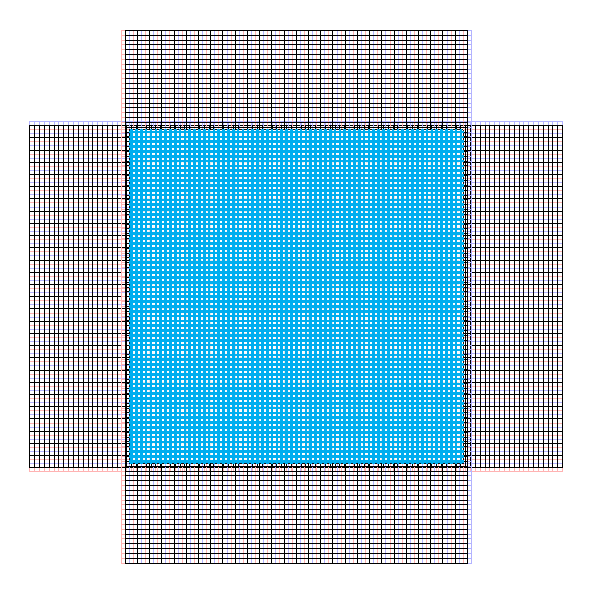
\includegraphics{op_concept.pdf}
    \caption[Overlaid model and data pixel grids]{The figure shows a basic IFU data set consisting of six
        exposures. First three are taken with the slices aligned in the
        $x$-direction; the light red and blue grids are offset wrt the black
        one by $\pm 6.9\,$mas in the $y$-direction. The rectangular pixels
        (8.2\,mas and 20.7\,mas in the $x$- and $y$-directions, or along- and
        across slices, respectively) can be seen in the black grid. After
        rotation by 90~degrees the slices are aligned in the $y$-direction
        and offsets are applied in the $x$-direction.  The overlaid cyan
        grid shows the area covered by all six exposures. This area is to
        be reconstructed on square pixels of 8.2\,mas as shown.
    }
    \label{fig:op_concept}
\end{figure}

The algorithm described here is inspired by the spectro-perfectionism of Bolton \& Schlegel (2010, \cite{bs10}).

We start with a forward model
\begin{equation}
  \label{eq:forward_model}
  \vec{d} = \mat{A}\vec{m} + \vec{e},
\end{equation}
where $\vec{d}$ and $\vec{m}$ are the data images and the model image, respectively,
both written as one-dimensional arrays (the six data images are collated into one array
$\vec{d}$).\footnote{The mapping from two-dimensional to one-dimensional arrays is in
principle arbitrary and can be chosen such that the model matrix $\mat{A}$ has a convenient form.
For the time being, the code uses the numpy method \lstinline{flatten()},
which returns the array as it is stored in computer memory.}
The vector $\vec{e}$ is the irreducible noise vector.
The data $\vec{d}$ are sampled on rectangular pixels $8.2 \times 20.7\,\mathrm{mas^{2}}$,
while the model $\vec{m}$ is constructed to be sampled on square pixels $8.2 \times 8.2\,\mathrm{mas^{2}}$
and aligned with the short side of the data pixels.
The model matrix $\mat{A}$ describes how the model flux is distributed onto the data grid.

A matrix element $\mat{A}_{ij}$ thus gives the geometric fraction of model pixel $j$ that overlaps with the data pixel $i$.
Fig.~\ref{fig:pixel_overlap} shows the situation for pixels that overlap completely in the $x$-direction.
In the code, we allow for partial overlap in the $x$-direction as well, so that the matrix element is
\begin{equation}
    \mat{A}_{ij} = f(\delta x_{ij}; D_{dx}, D_{mx}) f(\delta y_{ij}; D_{dy}, D_{my}),
    \label{eq:model_matrix_element}
\end{equation}
where $\delta x_{ij}$ and $\delta y_{ij}$ are differences in horizontal and vertical positions
of the data and model pixels and $D_{dx}$, $D_{dy}$, $D_{mx}$ and $D_{my}$ are the width and height
of the pixels in the data and model grids, respectively.

The function $f$ is given by
\begin{equation}
    \label{eq:overlap}
    f(\delta; D_{d}, D_{m}) =
        \begin{cases}
            \quad 1,
                & \text{if}\quad\abs{\delta} \leq \frac{D_{d} - D_{m}}{2} \\
            \frac{D_{d} + D_{m}}{2D_{m}} - \frac{1}{D_{m}}\abs{\delta},\quad
                & \text{if}\quad\frac{D_{d} - D_{m}}{2} < \abs{\delta} < \frac{D_{d} + D_{m}}{2} \\
            \quad 0,
                & \text{if}\quad\lvert{\delta} \geq \frac{D_{d} + D_{m}}{2}
        \end{cases}
\end{equation}

\begin{figure}
    \centering
    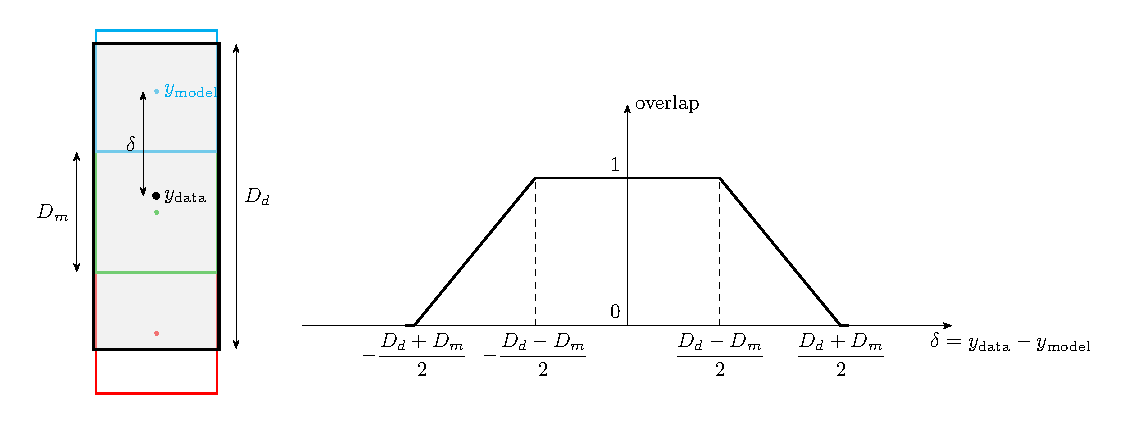
\includegraphics[width=\textwidth]{pixel_overlap.pdf}
    \caption[One-dimensional overlap as a function of pixel offset]{%
        The left panel shows a data pixel of size $D_{m}\times D_{d}$,
        overlapping with three model pixels of size $D_{m}\times D_{m}$.
        The pixels are aligned in the $x$-direction, so the overlap
        (which gives the matrix element of the model matrix $\mat{A}$)
        depends only on the distance $\delta = y_{\mathrm{data}} - y_{\mathrm{model}}$
        of the pixel centres through a stepwise linear function as shown on the right and given in Eq.~\eqref{eq:overlap}.
    }
  \label{fig:pixel_overlap}
\end{figure}

In the case if there is significant field rotation during
the observation and the data and model pixel grids are not aligned,
a more complex algorithm for determination of overlap must be used:

\begin{enumerate}
    \item For each pair of data and model pixels, the distance between their centres is computed.
        If it is larger than $\frac{1}{2}\sqrt{\left(D_{dx} + D_{mx}\right)^2 + \left(D_{dy} + D_{my}\right)^2}$,
        there is certainly no overlap and the computation may proceed with the next pair.
    \item Otherwise, the overlap is computed as follows:
        Since both pixels are rectangles, the overlap is guaranteed to be a convex polygon
        with at most eight distinct vertices, including degenerate cases with zero
        area: no overlap, a single point or a line segment.
    \item For each pair of rectangular pixels there are a total of 24 candidate vertices:
        \begin{itemize}
            \item Each vertex of a data pixel is also a vertex of the overlap polygon,
                if and only if it lies within the model pixel (4 candidate vertices).
            \item Each vertex of a model pixel is also a vertex of the overlap polygon,
                if and only if it lies within the data pixel (4 candidate vertices).
            \item Each intersection of an edge of a data pixel with an edge of a model pixel
                is necessarily a vertex of the overlap polygon ($4 \times 4 = 16$ candidate vertices).
        \end{itemize}
    \item The coordinates of the barycentre of the vertices are found
        as the arithmetic mean of their $x$ and $y$ coordinates.
    \item The vertices are ordered by their azimuth from the barycentre,
        in order to ensure that the resulting shape is a simple polygon.
    \item The area of the polygon $S$ is found as the sum of area of all triangles
        formed by the barycentre and all consecutive pairs of vertices
        using the shoelace formula or its equivalent, namely
        \begin{equation}
            2S = \sum\limits_{i = 0}^{n - 1} x_i \left(y_{i - 1} - y_{i + 1}\right),
        \end{equation}
        where all indices are mod $n$, the number of vertices in the polygon.
\end{enumerate}

Due to the presence of noise $\vec{e}$ in Eq.~\eqref{eq:forward_model},
a solution through direct inversion of the model matrix $\mat{A}$ is not possible.
A solution can, however, be obtained through $\chi^{2}$ minimisation:
\begin{equation}
    \chi^{2} = (\vec{d} - \mat{A}\vec{m})^{\mathrm{T}}\mat{C}^{-1}(\vec{d} - \mat{A}\vec{m}) \stackrel{!}{=} \mathrm{min}
    \label{eq:chi2_minimisation}
\end{equation}
Here, $\mat{C}$ is the covariance matrix, which describes the noise properties of the data.
The minimisation problem is solved analytically by
\begin{equation}
    \label{eq:chi2_solution}
    \vec{\hat{m}} = (\mat{A}^{\mathrm{T}}\mat{C}^{-1}\mat{A})^{-1}\mat{A}^{\mathrm{T}}\mat{C}^{-1}\vec{d} \equiv \mat{S}\vec{d}
\end{equation}

In the case of the METIS IFU the data vector $\vec{d}$ has $6 \times 100 \times 28 = 16800$ components.
The model has $68\times 68 = 4624$ components (the blue grid in Fig.~\ref{fig:op_concept}),
so the matrix $\mat{A}$ has $16800 \times 4624$ components.
The $4628 \times 16800$ solution matrix $S$ depends on the data
through the covariance matrix $\mat{C}$. Since the reconstruction operates on rectified IFU cubes,
i.e.~data that have been resampled from the raw data,
the pixel noises are correlated and $\mat{C}$ is non-diagonal.
As an approximation, the pixel noises could be treated as uncorrelated, in which case $\mat{C}$ would be diagonal.
If $\mat{C}$ were further approximated by the unit matrix (giving an unweighted least-squares reconstruction),
$\mat{S}$ would be independent of the data and could be reused and even be provided as a static calibration in the METIS pipeline.

\subsection{Data rates}
\label{ssec:criticalifudatarate}
\label{ssec:ifu_data_rate}

\begin{table}[ht]
  \centering
  \caption{Data rates}\label{tab:data_rates}
  \begin{tabular}{|l|r|r|c|c|}
    \hline
    \multicolumn{1}{|c|}{\textbf{Observing mode}} & \multicolumn{1}{c|}{\textbf{Max.\ rate}} & \multicolumn{1}{c|}{\textbf{Max.\ volume}} & \multicolumn{1}{c|}{\textbf{Night fraction}} & \multicolumn{1}{c|}{\textbf{Exp.\  volume}} \\
    \multicolumn{1}{|c|}{ }                       & \multicolumn{1}{c|}{[MiB s$^{-1}$]}     & \multicolumn{1}{c|}{[TiB]}                & \multicolumn{1}{c|}{[per 10h night]}         & \multicolumn{1}{c|}{[TiB]}                \\
    \hline\hline
    \textbf{Imager}                               &                                         &                                           &                                              &                                           \\
    IMG\_LM (burst mode)            & 200         & 5.49        & 0.10       & 0.55                                      \\
    IMG\_N (burst mode)             & 182         & 4.99        & 0.10       & 0.50                                      \\
    IMG\_N  (half-cycle average)    & 32          & 0.88        & 0.00       & 0.00                                      \\
    IMG\_LMN  (parallel mode)       & 382         & 10.49       & 0.10       & 1.05                                      \\
    \hline
    \textbf{Spectroscopy}          &                            &                      &                  &                                           \\
    SPEC\_LM                       & 200         & 5.49         & 0.05       & 0.27                       \\
    SPEC\_N                        & 182         & 4.99         & 0.05       & 0.25                       \\
    SPEC\_LMN  (parallel mode)     & 382         & 10.49        & 0.06       & 0.63                                      \\
    IFU + IMG\_LM parallel (IFU)   & 64          & 1.76         & 0.54       & 1.25                       \\
    IFU + IMG\_LM parallel (IMG)   & 200         & 5.49         & 0.54       & 2.67                                      \\
    \hline
  \end{tabular}
\end{table}


Observing with the shortest possible exposure times, for bright targets,
results in high data rates (cf.~Table~\ref{tab:data_rates}, values taken from
\cite{METIS-data_rates}). This is a potential problem for the observatory
pipeline which has to deal with the data in semi-real time, meaning that no
backlog of pending data reductions should accumulate.

However, the maximum estimated data rate for a single mode has decreased by a
factor of four between PDR and FDR because the rate by which the IFU detectors
can be read out has been decreased. This helps ameliorate the issue. 
The fastest frame rate will be 1 Hz.
Sources that would need faster frame rates will be observed with a coronagraph and/or a ND filter.

In addition, the observatory pipeline does not have to perform a full data reduction
as described in Sect.~\ref{sssec:ifu_sci_process}, but foremost compute a number
of quality control parameters to assess the quality of the data and a
"quick-look" at the data for the observers. In the course of the development of
the observatory recipes, the details on how individual parts of the pipeline
perform will become clear and there will be enough freedom in the choice of
parameters to, if necessary, reduce the performance of the recipe if a high data
stream is to be expected. Another option might be to compute QC parameters only
on a subset of incoming frames.


This is in compliance with \REQ{METIS-6075}.


% Additional critical algos
\subsection{ADI algorithm}\label{ssec:criticaladialgorithm}
Considering many of the science cases for METIS are focusing on direct imaging / high contrast imaging we deem it critical that we demonstrate that METIS-like data can be ADI-reduced without major issues.
ADI reduction with focal plane and pupil plane coronagraphs, in addition to ADI+SDI with the IFU (partially spatially undersampled with an additional spectral dimension) is therefore demonstrated.
It is recognized that the required techniques are already known from earlier publications of data collected with high contrast imagers and AO-fed IFUs.
This study allows the PIP team to become more familiar with them and to present prototype algorithms in a centralized location.

\subsubsection{Generation of representative set of IMG\_LM data: planetary system}
Using a combination of the HEEPS code and the ScopeSim code with the METIS package we have performed simulations of a star and a point source companion in order to test critical algorithms for high contrast imaging on simulated data of METIS.
Using the HEEPS code we simulate a sequence of up to 12000 PSFs of an unresolved star behind the RAVC coronagraph and of an unresolved companion sufficiently far away from the coronagraph to be considered off-axis, with each PSF corresponding with an integration time of 300 milliseconds for a total of 3600 seconds of observing time. Each PSF is generated with a (SCAO-only) wavefront sampled every 300 ms (comparable to the coherence time t0 at L-band), thereby effectively time sampling the atmospheric wavefront aberrations. Both PSFs are scaled to the magnitude of the parent star ($L=3.5$). For this demonstration we use a time sequence of 12000 PSFs but will apply some windowing and temporal binning to increase execution speed on a laptop. 
The two PSFs are combined together with an offset of 100 mas, an additional delta magnitude ($\Delta L=7.7$) for the companion and field rotation over 1 hour (corresponding with 30 degrees change in position angle). The system could be described at Beta Pic b orbiting at 100 mas around its host star. A second source is added at opposite position angle to see the symmetry of the reduction (of use for the APP coronagraph which only has one dark hole). This combined source is fed into ScopeSim as a fits file with the WCS information conveying the spatial extent. The coronagraphic transmissions are transferred to ScopeSim as well during this process.
In the ScopeSim step the instrumental noise and background expected from both METIS and ELT is injected and the source flux reduced according to system transmission. 
After these processing steps we are left with a large 3D cube of a star (x, y, time) with two planets undergoing field rotation which we use for the ADI processing step using the VIP\_HCI package. For this example, the output images have been truncated to 201x201 pixels and the images have been binned to 30 seconds exposure time ($N_\mathrm{bin}=100$) to further reduce execution time.
\subsubsection{Demonstration of ADI algorithm on simulated IMG\_LM data}
The most basic PSF subtraction of VIP\_HCI is the standard ADI algorithm from Marois et al 2006, where the median of the cube is first subtracted and in a second step optimally-scaled time-localized medians are subtracted in annular rings. Afterwards each image in the cube is derotated with the known position angle. Subsequently the derotated and PSF subtracted images are averaged to give a final stacked version. When the second annular optimized subtraction step is skipped this procedure is equal to the one described in the PIP Spec.
For the IFU, this ADI procedure can similarly be followed for each wavelength in the reduced cubes. In VIP\_HCI it is possible to do a two-step (first ADI then SDI) or single-step reduction, in which rescaled images from other wavelength slices are used to provide additional PSF reference material.
Example output images for ADI reduction for LM RAVC data.


\begin{figure}[!ht]
  \centering
  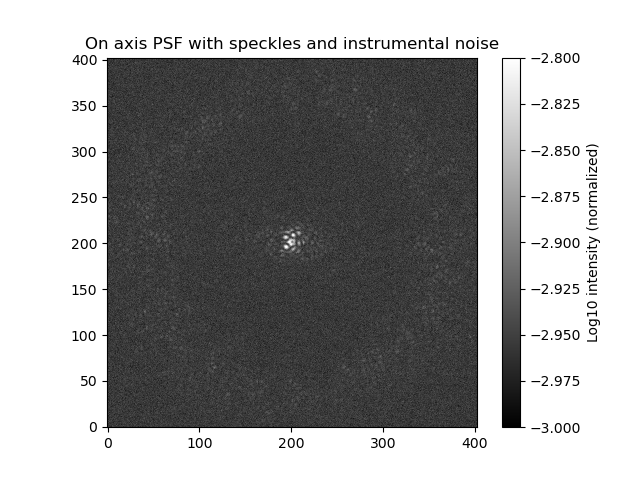
\includegraphics[width=0.6\textwidth]{./figures/onaxis_psf.png}
  \caption{On-axis coronagraphic PSF with instrumental noise injected and with corrected atmospheric turbulence. The circular control region from the AO system is clearly visible.}
  %\label{fig:metis_l}
\end{figure}
\begin{figure}[!ht]
  \centering
  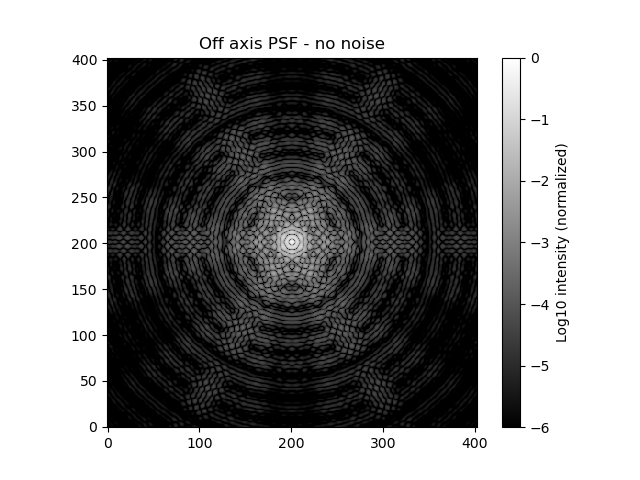
\includegraphics[width=0.6\textwidth]{./figures/offaxis_psf.png}
  \caption{Off-axis PSF without instrumental noise.}
  %\label{fig:metis_l}
\end{figure}

\begin{figure}[!ht]
  \centering
  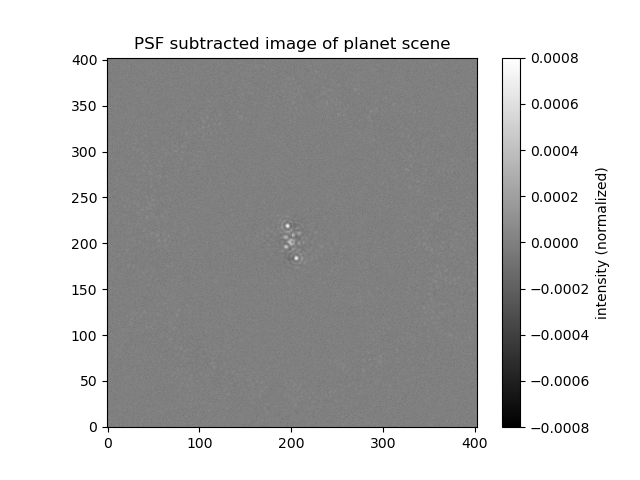
\includegraphics[width=0.6\textwidth]{./figures/adi_meansub.png}
  \caption{Single frame of image stack with mean PSF subtracted.}
  %\label{fig:metis_l}
\end{figure}

\begin{figure}[!ht]
  \centering
  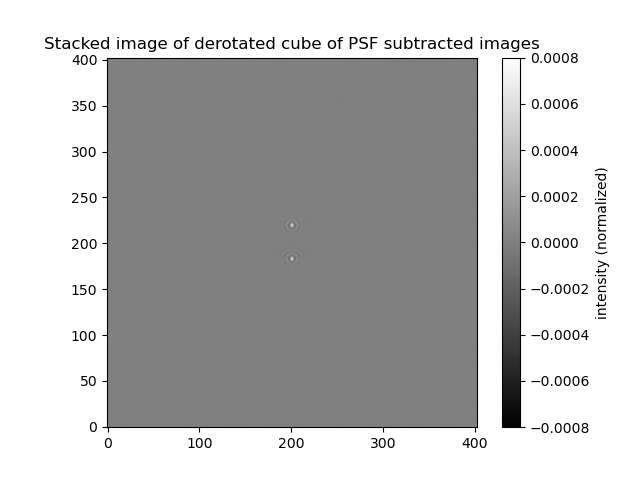
\includegraphics[width=0.6\textwidth]{./figures/adi_derotstack.png}
  \caption{Derotated stack of ADI reduced images.}
  %\label{fig:metis_l}
\end{figure}

Additionally, the contrast curves can be extracted (raw contrast over time-averaged cube, 5 sigma contrast after ADI processing). Please note that the plotted contrast is dependent on the assumptions made for this demonstration (SCAO-only effects, no additional jitter / pupil drifts / no residual atmospheric dispersion, 120 binned frames with each 100 frames of 0.3s integration time, 30 degrees image rotation). 
Injection and retrieval of point sources of known intensity is performed to calculate the efficiency or throughput of the ADI post-processing technique. Closer to the star the same amount of position angle movement will be seen as an increasingly smaller physical movement. Therefore, self-subtraction of a point source signal will be more pronounced and increased losses are seen close to the star. The following plot shows the post-processing only component of the ADI reduction losses. The radial coronagraphic throughput losses due to partial suppression of off-axis sources will be provided separately (and is not included in these sensitivity plots for this example).



Following the SNR definitions of Mawet et al 2014 the noise is calculated in annular rings and corrected for the relatively low number of effective samples. A 5-sigma sensitivity curve is produced by injection and retrieval of sources. In addition, a post-ADI SNR map is generated. Note that the two injection planets are so bright that an unmasked SNR map gives an underestimated SNR as their presence strongly alters the local noise estimate. Nonetheless they are both recognized as significant detections.

\begin{figure}[!ht]
  \centering
  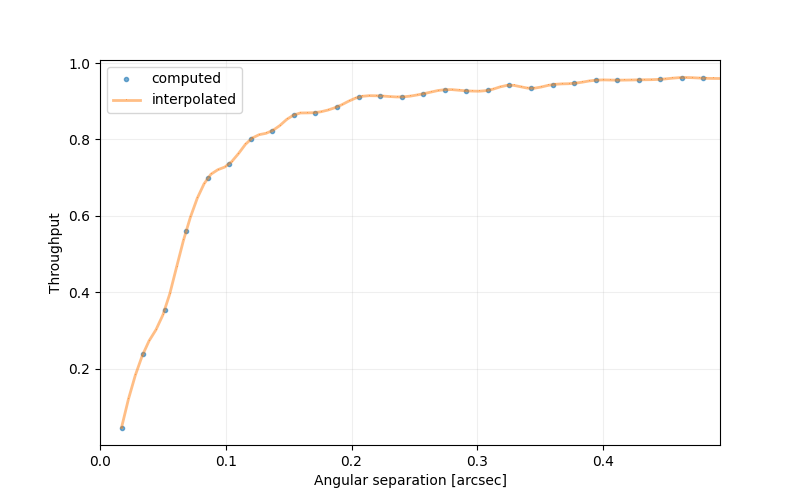
\includegraphics[width=0.6\textwidth]{./figures/adi_throughput.png}
  \caption{Efficiency of ADI algorithm in retrieving inserted point sources as a function of angular separation.}
  %\label{fig:metis_l}
\end{figure}

\begin{figure}[!ht]
  \centering
  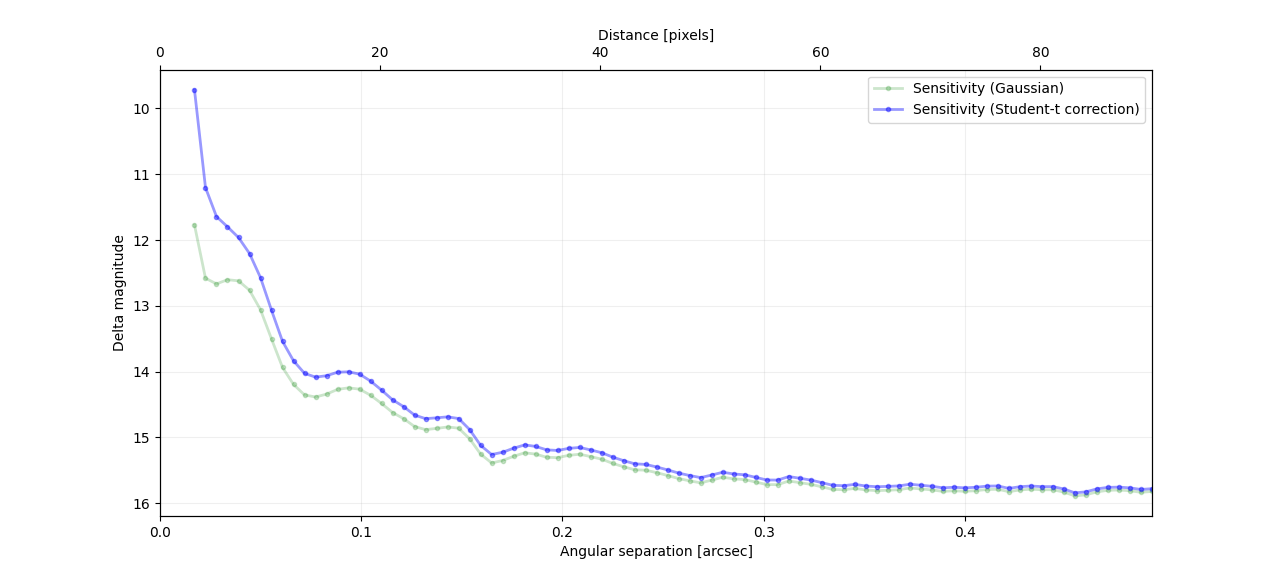
\includegraphics[width=0.6\textwidth]{./figures/adi_contrast.png}
  \caption{Achievable contrast for the $L=3.5$ target in 1 hour integration time as a function of angular separation.}
  %\label{fig:metis_l}
\end{figure}

\begin{figure}[!ht]
  \centering
  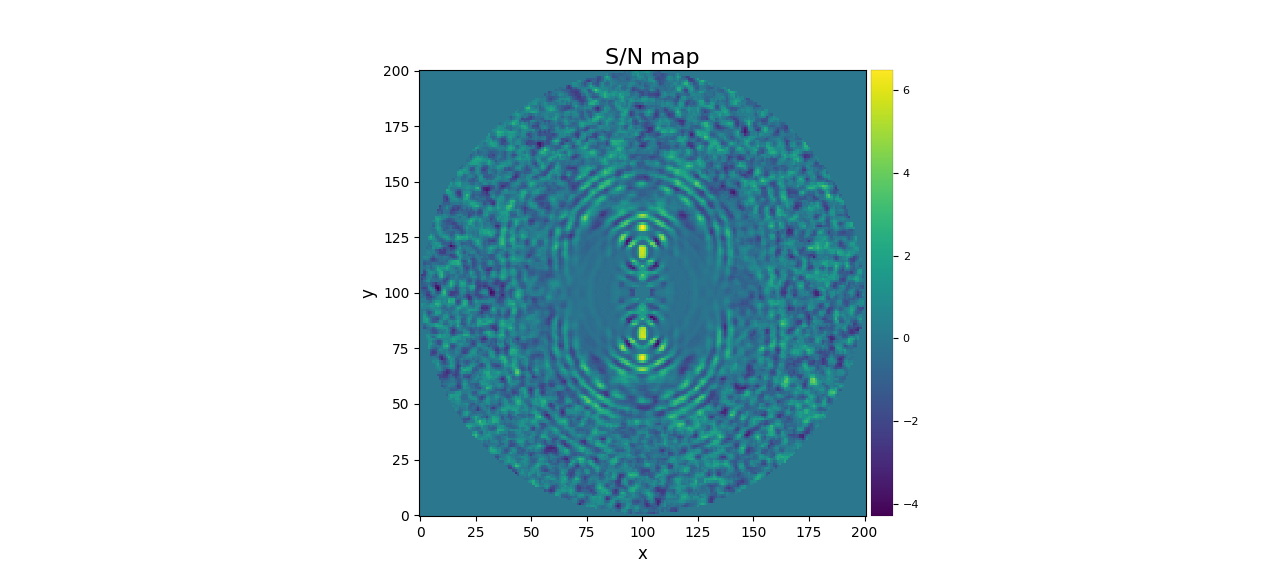
\includegraphics[width=0.6\textwidth]{./figures/adi_snrmap.png}
  \caption{Two dimensional ADI map of post ADI signal to noise of point sources. Two point sources that were inserted at 100 mas are seen.}
  %\label{fig:metis_l}
\end{figure}

\subsubsection{Generation of representative set of IFU data}

To demonstrate the ADI/SDI reduction of an IFU dataset which contains spatial, temporal and spectral information we first generate a METIS IFU HCI dataset of 12000 frames by 267 by 267 pixels and Z spectral bins. Each frame corresponds with an exposure time of 0.3 seconds, with a total integration time of 1 hour.  
We generate PSFs with the HEEPS python code in L band with the RAVC coronagraph at a pixel scale of 8.2 by 8.2 mas. At a central wavelength of 3.8 micron this corresponds to approximately 100 by 100 lambda/D. This data is FFT interpolated with VIP\_HCI with a scaling factor to generate 1600 spectral bins in a wavelength range of X micron at a wavelength of X micron. 
As the METIS IFU projected on-sky has rectangular pixels we average the data in one dimension to get a pixel scale of 8.2 by 24.6 mas (note actual scale is close to 8.2 x 21 mas). The sum of all flux is set to be equal to the total photons of the star in L-band.
To go back to square pixels, we duplicate the undersampled axis. We inject noise according to the shot noise of the source, sky background and detector read noise with a single resolution element spanning about x by x pixels, while also using a binning factor of X spectrally and 100 temporally to reduce memory consumption.



 


\subsubsection{Demonstration of ADI+SDI algorithm on IFU data}


This dataset is used together with an array containing a set of position angles given 1 hour of sky rotation and an array containing the wavelengths of the spectral axis to perform a median PSF subtraction technique using VIP\_HCI on the generated data. This is a two-step process where first for each timestep all spectral slices are rescaled to be on the same lambda/D grid. Then the median of the cube in the spectral dimension is subtracted. This is repeated for every timestep to give a time varying array of residuals. For this array the median in time is also calculated and subtracted. Afterwards the residuals are derotated and stacked and analysed yielding the following 5 sigma performance curves. 

[insert images of IFU ADI+SDI data reduction]
